\documentclass[a4paper,12pt]{amsart}

\newcommand{\ZZ}{\mathbb{Z}}
\newcommand{\RR}{\mathbb{R}}
\newcommand{\CC}{\mathbb{C}}
\newcommand{\PP}{\mathbb{P}}
\newcommand{\bfx}{\mathbf{x}}
\newcommand{\bfy}{\mathbf{y}}
\newcommand{\bfb}{\mathbf{b}}
\newcommand{\vx}{\begin{bmatrix}
		x_1\\
		\vdots\\
		x_n
\end{bmatrix}}
\newcommand{\vA}{\begin{bmatrix}
		A\\
		-A\\
		-I
\end{bmatrix}}
\newcommand{\bb}[1]{{\mathbb{#1}}}
\newcommand{\mc}[1]{{\mathscr{#1}}}
\newcommand{\tens}[1]{%
	\mathbin{\mathop{\otimes}\displaylimits_{#1}}%
}
\newcommand{\fk}{\mathfrak}

\newcommand{\OO}{\ensuremath{\mathcal{O}}}
\newcommand{\m}{\ensuremath{\mathfrak{m}}}
\newcommand{\p}{\ensuremath{\mathfrak{p}}}

\newcommand{\xra}{\ensuremath{\xrightarrow}}
\newcommand{\C}{\ensuremath{\mathbb{C}}}
\newcommand{\R}{\ensuremath{\mathbb{R}}}
\newcommand{\Z}{\ensuremath{\mathbb{Z}}}
\newcommand{\Q}{\ensuremath{\mathbb{Q}}}
\newcommand{\HH}{\ensuremath{\mathbb{H}}}
\newcommand{\I}{\ensuremath{\mathds{1}}}
\newcommand{\ot}{\ensuremath{\otimes}}
\newcommand{\del}{\ensuremath{\mathbb{P}artial}}
\newcommand{\iv}{\ensuremath{^{-1}}}
\newcommand{\bs}{\ensuremath{\backslash}}
\newcommand{\con}{\ensuremath{\bigtriangledown}}
\newcommand{\ra}{\ensuremath{\xrightarrow}}
\newcommand{\gr}{\ensuremath{\nabla}}
\newcommand\rd[1]{{\color{red}#1}}
\newcommand\bl[1]{{\color{blue}#1}}
\newcommand{\iif}{\ensuremath{\Leftrightarrow}}
\newcommand{\mf}{\ensuremath{\mathfrak}}

\newcommand\restr[2]{{% we make the whole thing an ordinary symbol
		\left.\kern-\nulldelimiterspace % automatically resize the bar with \right
		#1 % the function
		\vphantom{\big|} % pretend it's a little taller at normal size
		\right|_{#2} % this is the delimiter
}}
\DeclareMathOperator{\Aut}{Aut}
\DeclareMathOperator{\Inn}{Inn}
\DeclareMathOperator{\Hom}{Hom}
\DeclareMathOperator{\Spec}{Spec}

\usepackage[top=1in, bottom=1in, left=1in, right=1in]{geometry}
\usepackage{amsmath, amssymb}
\usepackage{amsthm}
\usepackage{dsfont}
\usepackage{enumerate}
\usepackage{graphicx}
\usepackage{tikz-cd}
\usepackage{subcaption}

\makeatletter
\newcommand\xleftrightarrow[2][]{%
	\ext@arrow 9999{\longleftrightarrowfill@}{#1}{#2}}
\newcommand\longleftrightarrowfill@{%
	\arrowfill@\leftarrow\relbar\rightarrow}
\makeatother


\title{MATH7670 Lecture Notes}
\author{}


\date{January 24, 2019}
\begin{document}
\maketitle
\newtheorem{Lemma}{Lemma}
\newtheorem{Proposition}{Proposition}[section]
\newtheorem{Theorem}{Theorem}[section]
\newtheorem{Corollary}{Corollary}
\newtheorem*{Conjecture}{Conjecture}

\theoremstyle{definition}
\newtheorem*{Problem}{Problem}
\newtheorem*{Def}{Definition}
\newtheorem{Eg}{Example}[section]
\newtheorem*{exercise}{Exercise}

\theoremstyle{remark}
\newtheorem*{Remark}{Remark}
\newtheorem*{Caution}{\bf{Caution}}
\newtheorem*{Fact}{Fact}
\newtheorem*{Note}{Note}

%---This is the beginning of the document---

\section{Lecture 01}

What is a toric variety(over $\CC$)? simplest: $\PP^n$, also $\PP^{n_1}\times\PP^{n_2}\times\dots\times\PP^{n_r}$(via Segre embdedding).

\begin{Eg}[Hirzebruch surface]
A polygon
\begin{figure}[h]
\centering
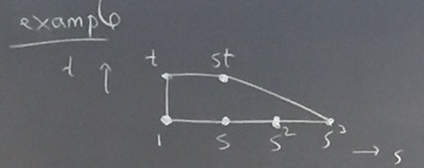
\includegraphics[width=0.7\textwidth]{pic/lec01pic01}
\end{figure}
\begin{align*}
\varphi:\mathbb{A}^2_{s,t}&\rightarrow\PP^5\\
(s,t)&\mapsto(1,s,s^2,s^3,t,st)
\end{align*}
Consider
\begin{equation*}
\overline{\varphi(\mathbb{A}^2)}=X\subseteq\PP^5.
\end{equation*}
$X$ is an example of a toric variety.
The edges correspond to curves $C_1,\dots,C_4$ on $X$, $C_1\cap C_2=\text{pt}$, $C_2\cap C_3=\text{pt}$, etc. $\text{Pic}X$ is generated by $[C_1],[C_2]$
\end{Eg}
Toric varieties allow explicit constructions of many concepts in A.G.
\begin{itemize}
\item singularities, smoothness, resolution of singularities 
\item divisors, geometry of divisors $\text{Pic}X$, $\text{Cl}X$.
\item cohomology of divisors
\item vector bundles, projective bundles, sheaf of differentials
\item  Serre duality, Riemann-Roch
\end{itemize}

Special features:
\begin{itemize}
\item defined using: cones, fans, polyhedron
\item action of the torus
\begin{equation*}
T=(\CC^*)^n.
\end{equation*}
\item homogenerous coordinates on a toric variety.
\end{itemize}

\begin{Caution}
Our toric varieties are always normal.
\end{Caution}
First few weeks:
\begin{itemize} 
\item cones, F-M,
\item affine toric varieties: define/ideals/points/singularities, maps, T-action.
\item projective, more general, toric varieties
\end{itemize} 
\subsection{Cones}
Let $V$ be a finite dimensional $\RR$-vector space.
\begin{Def}
Let $S\subseteq V$ be a subset, nonempty.
\begin{enumerate}
\item $S$ is a \textbf{(convex) cone} if $\forall \bfx,\bfy\in S$, $\forall \alpha,\beta\in\RR$, $\alpha,\beta\geq 0$, then $\alpha \bfx+\beta \bfy\in S$.
\item $S$ is a \textbf{convex set} if $\forall \bfx,\bfy\in S$, $\forall \alpha,\beta\in\RR$, $\alpha,\beta\geq 0$, $\alpha+\beta=1$, then $\alpha \bfx+\beta \bfy\in S$.
\end{enumerate}
\end{Def}
\begin{Eg}Some examples when $V=\RR^2$:
\begin{enumerate}
\item A convex cone:
\begin{figure}[h]
\centering
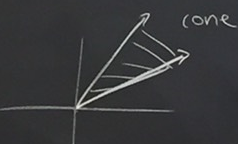
\includegraphics[width=0.7\textwidth]{pic/lec01pic02a}
\end{figure}
\item Convex sets:
\begin{figure}[h]
\centering
\begin{subfigure}{.5\textwidth}
  \centering
  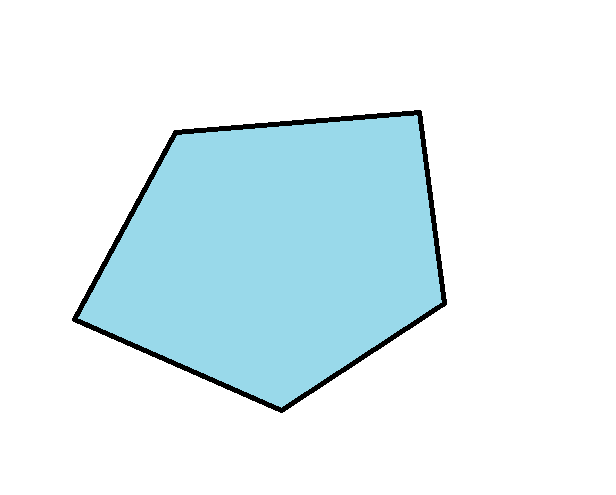
\includegraphics[width=.7\linewidth]{pic/lec01pic02b}
  \caption{A polygon}
  \label{fig:sub1}
\end{subfigure}%
\begin{subfigure}{.5\textwidth}
  \centering
  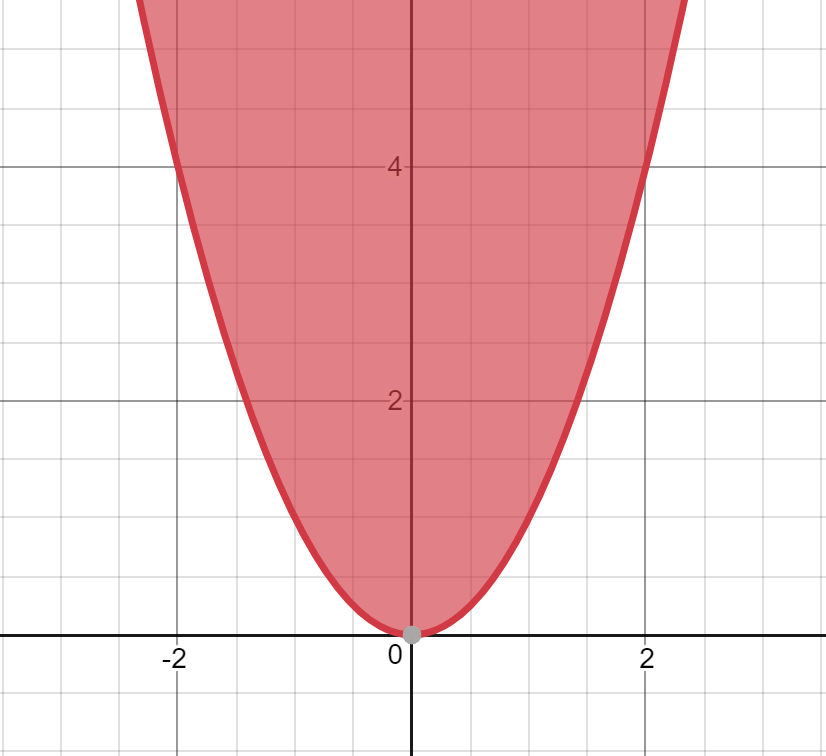
\includegraphics[width=.7\linewidth]{pic/lec01pic02c}
  \caption{$y\geq x^2$}
  \label{fig:sub2}
\end{subfigure}
\label{fig:test}
\end{figure}
\end{enumerate}
\end{Eg}

\begin{Eg}Key examples:
\begin{enumerate}
\item If $A\in \RR^{m\times n}$, write $A=[A_1, A_2\dots, A_n]$, define
\begin{align*}
\text{vcone}(A)&:=\{x_1A_1+\dots+x_nA_n\in\RR^n,x_1,\dots,x_n\geq 0\}\\
&=\{A\bfx\in\RR^n: \bfx\geq 0, \bfx\in \RR^n\}
\end{align*}
A cone of this form is called finitely generated or V-cone.
\item obtain cone via intersections of half-spaces. If
\begin{align*}
B=\begin{bmatrix}
B_1\\
\vdots\\
B_d
\end{bmatrix}, B_i\in(\RR^n)^{*}
\end{align*}
Define
\begin{align*}
\text{hcone}(B)&:=\{\bfy\in(\RR^n)^{*}:\langle B_1,\bfy \rangle=B_1\bfy\leq 0,\dots,\langle B_n,\bfy \rangle=B_n\bfy\leq 0\}\\
&=\{\bfy\in(\RR^m)^*:B\bfy\leq 0\}
\end{align*}
\item if $A\in\RR^{m\times n}$, define
\begin{equation*}
\text{conv}(A):=\{x_1A_1+\dots+x_nA_n:x_i\geq 0,\sum x_i=1\}
\end{equation*}
A set of this form is a polytope.
\item if $A\in\RR^{m\times n}$, $\bfb\in\RR^m$
\begin{equation*}
P(A,\bfb):=\{\bfx\in\RR^n:A\bfx\leq \bfb\}
\end{equation*}
A set of this form is a polyhedron.
\end{enumerate}
\end{Eg}
\begin{Def}[Key construction: dual cone]
If $\sigma\in V$ is a cone, define its \textbf{dual cone}
\begin{align*}
\sigma^{\vee}=\{\bfy\in V^{*}:\langle \bfy,\bfx\rangle\leq 0, \forall \bfx\in\sigma\}.
\end{align*} 
(Check: $\sigma^{\vee}$ is also a cone.)
\end{Def}

\begin{Eg}
$V=\RR^2$. Let $\sigma=\text{cone}(A_1,A_2)$. Then $\sigma^{\vee}=\text{cone}(A_1^{\perp},A_2^{\perp})$.
\begin{figure}[h]
\centering
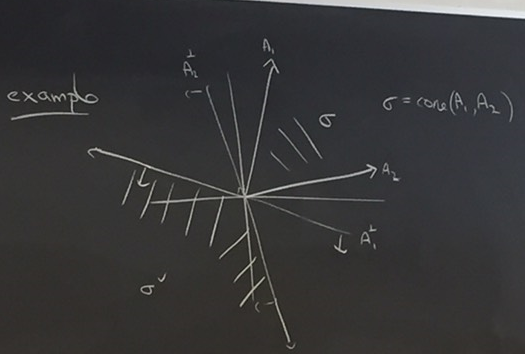
\includegraphics[width=0.7\textwidth]{pic/lec01pic03}
\end{figure}
\end{Eg}
\begin{Remark}
if $\sigma=\text{vcone}(A)$, $A\in\RR^{m\times n}$, then $\sigma^{\vee}=\text{hcone}(A^{T})$. This is because
\begin{align*}
\sigma^{\vee}&=\{\bfy\in(\RR^m)^*:\langle \bfy,\bfx \rangle\leq 0,\forall \bfx\in \sigma\}\\
&=\{\bfy: \langle \bfy,A_1 \rangle\leq 0,\dots,\langle \bfy,A_n \rangle\leq 0\}.
\end{align*}
\end{Remark}
Some desires:
\begin{enumerate}
\item show that $\sigma$ is a hcone$\iff$ $\sigma$ is a vcone
\item  find $\sigma^{\vee}$, i.e. find $B$ s.t. $\sigma^{\vee}=\text{vcone}(B)$
\item $\sigma^{\vee\vee}=\sigma$ ?
\end{enumerate}

\subsection{Fourier-Motzkin elimination}
Let $\text{vcone}(A)=\{A\bfx:\bfx\geq 0\}$, consider
\begin{align*}
C&=\{\begin{bmatrix}\bfx\\\bfy\end{bmatrix}:\bfx\in\RR^n,\bfy\in\RR^m,\bfy=A\bfx,\bfx\geq 0\}\\
&=\{\begin{bmatrix}\bfx\\\bfy\end{bmatrix}:\begin{bmatrix}
A& -I\\
-A& I\\
-I& 0
\end{bmatrix}\begin{bmatrix}\bfx\\\bfy\end{bmatrix}\leq 0\}
\end{align*} 
is an hcone $\subseteq\RR^{n+m}$. Consider $\pi_\bfy$
\begin{align*}
\pi_\bfy:\RR^{n+m}&\rightarrow\RR^{m},\\
\begin{bmatrix}\bfx\\\bfy\end{bmatrix}&\mapsto \bfy.
\end{align*}
Then $\pi_\bfy(C)=\sigma$.\\
Generalize: let $P=P(A,\bfb)=\{\bfx\in \RR^n: A\bfx\leq \bfb\}\subseteq \RR^n$. Fix $1\leq k\leq n$ column index ($A\in\RR^{m\times n}$), define
\begin{align*}
\pi_k:\RR^n&\rightarrow \RR^n\\
\begin{bmatrix}x_1\\ \vdots \\ x_n\end{bmatrix}&\mapsto \begin{bmatrix}
x_1\\
\vdots\\
0\\
\vdots\\
x_n
\end{bmatrix}.
\end{align*}
The image of $\pi_k$ is $\{x_k=0\}=\RR^{n-1}\subseteq\RR^n$. Then $\pi_k(P)\subseteq\RR^{n-1}\subseteq\RR^n$. Is $\pi_k(P)$ a polyhedral? 
\begin{Theorem}[Fourier-Motzkin elimination]
\label{Thm_FM}
Fix $A\in\RR^{m\times n}$, $1\leq k\leq n$, then there exists $C\in\RR^{r\times m}$, some $r$, s.t.
\begin{enumerate}
\item $C\geq 0$
\item $CA$ has column $k$ equal to $0$
\item  if $P=P(A,\bfb)$, then $\pi_k(P)=P(A',\bfb')$ where $A'=CA$, $\bfb'=C\bfb$.
\end{enumerate}
\end{Theorem}
\begin{Eg}
\begin{align*}
A=\begin{bmatrix}
1&1&-1\\
2&-1&-1\\
1&0&1\\
1&-2&0
\end{bmatrix},\sigma=\{\bfx: A\bfx\leq 0\}\subseteq\RR^3
\end{align*}
and
\begin{align*}
\pi_3:\RR^3\rightarrow\RR^3,\\
\begin{bmatrix}
x_1\\x_2\\x_3
\end{bmatrix}\mapsto\begin{bmatrix}
x_1\\x_2\\0
\end{bmatrix}
\end{align*}
\begin{equation}
\label{eqn*}
\begin{cases}
x_1+x_2-x_3\leq 0\\
2x_1-x_2-x_3\leq 0\\
x_1+x_3\leq 0\\
x_1-2x_2\leq 0
\end{cases}
\end{equation}
parition $\{1,2,3,4\}$:
\begin{align*}
Z&:=\{4\}\\
N&:=\{1,2\}\\
P&:=\{3\}
\end{align*}
\begin{equation}
\label{eqn**}
\begin{cases}
x_1-2x_2\leq 0\\
2x_1+x_2\leq 0\\
3x_1-x_2\leq 0
\end{cases}
\end{equation}
if $\begin{bmatrix}
x_1\\
x_2\\
0
\end{bmatrix}$ satisfies (\ref{eqn**}), find $\begin{bmatrix}
x_1\\
x_2\\
x_3
\end{bmatrix}$ satisfies (\ref{eqn*}):
\begin{align*}
x_3\geq x_1+x_2\\
x_3\geq 2x_1-x_2\\
x_3\leq -x_1
\end{align*}
Let 
\begin{align*}
L&=\max(x_1+x_2,2x_1-x_2),\\
U&=\min(-x_1),
\end{align*}
then any $x_3$ s.t. $L\leq x_3\leq U$ satisfies $\begin{bmatrix}
x_1\\x_2\\x_3
\end{bmatrix}\in\sigma$.
\end{Eg}

%---- Lecture 02 on Jan. 24th ---------
\newpage
\section{Lecture 02}
Recall: F-M elimination (Theorem\ref{Thm_FM}). (HW: prove it.)\\
We had defined $\sigma^{\vee}$: $\sigma\subseteq V=\RR^m$
\begin{align*}
\sigma^{\vee}=\{\bfy\in V^{*}:\langle \bfy,\bfx\rangle\leq 0, \forall \bfx\in\sigma\}.
\end{align*} 
Goals: 
\begin{itemize}
\item $\text{hcones}=\text{vcones}$
\item $\sigma^{\vee\vee}=\sigma$
\end{itemize}
\subsection{"Farkas jungle"}
\begin{Corollary}
\label{cor02_01}
Let $A\in\RR^{m\times n}$, $\bfb\in\RR^{m}$, then either
\begin{enumerate}
\item $\exists \bfx\in\RR^n$ s.t. $A\bfx\leq \bfb$, or
\item $\exists \bfy\in\RR^m$ s.t. $\bfy^TA=A^T\bfy=0$, $\bfy\geq 0$ but $\bfy^T\bfb=\langle\bfy,\bfb\rangle<0$,
\end{enumerate}
but not both.
\end{Corollary}
\begin{proof}
not both: If we have $A\bfx\leq \bfb$, $\bfy^TA=0$, $\bfy\geq 0$, $\bfy^T\bfb<0$, then
\begin{align*}
0=\bfy^TA\bfx\leq \bfy^T\bfb<0.
\end{align*}
Contradiction!\\
Suppose $A\bfx\leq \bfb$ has no solution. Produce $\bfy$:
Apply F-M to columns $n,n-1,\dots,1$, obtain $C\in\RR^{N\times m}$, $C\geq 0$ and $CA=0$.
Then we get a system $0=CAX\leq C\bfb=\bfb'$ having no solutions.
So some $b'_i=0$. Let $\bfy^T=$ $i$-th row of $C$. So
\begin{align*}
\bfy\geq 0,\\\bfy^TA=0,\\\bfy^T\bfb<0.
\end{align*}
\end{proof}

\begin{Corollary}
Let $A\in\RR^{m\times n}$, $\bfb\in \RR^m$, then either
\begin{enumerate}
\item $\exists \bfx\in\RR^n$ s.t. $A\bfx= \bfb$, $\bfx\geq 0$ or,
\item $\exists \bfy\in\RR^m$ s.t. $\bfy^TA\leq 0$, $\bfy^T\bfb> 0$,
\end{enumerate}
but not both.
\end{Corollary}
\begin{proof}
Not both: $A\bfx=\bfb$,
\begin{align*}
\bfy^TA\bfx=\bfy^T\bfb>0
\end{align*}
Contradiction!\\
Assume (1) fails, i.e.
\begin{equation*}
\{\bfx\in\RR^n:\begin{bmatrix}
A\\-A\\-I
\end{bmatrix}\bfx\leq\begin{bmatrix}
\bfb\\-\bfb\\0
\end{bmatrix}\}=\emptyset
\end{equation*}
by Corollary \ref{cor02_01}, $\exists \begin{bmatrix}
\bfy_1\\ \bfy_2\\ \bfy_3
\end{bmatrix}\geq 0$ s.t.
\begin{align*}
\begin{bmatrix}
\bfy_1^T& \bfy_2^T& \bfy_3^T
\end{bmatrix}\begin{bmatrix}
A\\-A\\-I
\end{bmatrix}=0,\\
\begin{bmatrix}
\bfy_1^T& \bfy_2^T& \bfy_3^T
\end{bmatrix}\begin{bmatrix}
\bfb\\-\bfb\\0
\end{bmatrix}<0,
\end{align*}
so
\begin{align*}
(\bfy_1^T-\bfy_2^T)A=\bfy_3^T\geq 0,\\
(\bfy_1^T-\bfy_2^T)\bfb< 0.
\end{align*}
Let $\bfy=\bfy_1^T-\bfy_2^T$.
\end{proof}

\begin{Corollary}[Farkas lemma]
Let $\sigma=\text{vcone}(A)$, $A\in\RR^{m\times n}$, let $\bfb\in \RR^{m}$, then either
\begin{enumerate}
\item $\bfb\in \sigma$ or,
\item $\exists \bfy\in\sigma^{\vee}$ s.t. $\bfy^T\bfb>0$.
\end{enumerate}
\end{Corollary}

\begin{Corollary}
Given $A\in\RR^{m\times n}$, $\bfb\in\RR^{m}$, let $\sigma=\text{vcone}(A)\subset\RR^m$. If $\bfb\not\in \sigma$, then $\exists \bfy\in\sigma^{\vee}\subseteq(\RR^n)^{*}$ s.t. $\bfy^T\sigma\leq 0$, $\bfy^T\bfb>0$. i.e.
\begin{align*}
	\sigma\subseteq H_{\bfy}^{\leq 0}:=\{\bfx\in\RR^m:\bfy^T\bfx\leq 0\}
\end{align*}
and
\begin{align*}
\bfb\in H_{\bfy}^{> 0}:=\{\bfx\in\RR^m:\bfy^T\bfx> 0\}.
\end{align*}
\end{Corollary}

Notation: $\bfy^{\perp}:=H_{\bfy}^{= 0}:=\{\bfx\in\RR^m:\bfy^T\bfx= 0\}$.

\begin{Corollary}
let $\sigma=\text{vcone}(A)\subseteq\RR^m$, $A\in\RR^{m\times n}$, then $\sigma=\sigma^{\vee\vee}$.
\end{Corollary}
\begin{proof}
\begin{enumerate}
\item $\sigma\subseteq\sigma^{\vee\vee}$: this is essentially formal.
\begin{align*}
\bfy\in\sigma^{\vee}\iff \bfy^TA_1\leq 0,\dots,\bfy^TA_n\leq 0\\
\iff \bfy\in\text{hcone}(A).
\end{align*}
need to show $A_i\in\text{hcone}(A^T)^{\vee}=\sigma^{\vee\vee}$, if $\bfy\in\sigma^\vee$, then $\bfy^TA_i\leq 0$ $\implies$ $A_i\in\sigma^{\vee\vee}$.
\item  $\sigma\supseteq\sigma^{\vee\vee}$ is the main part:\\
If $\bfb\in\sigma^{\vee\vee}$, but $\bfb\not\in\sigma$,
Farkas $\implies$ $\exists \bfy\in\sigma^{\vee}$ s.t. $\bfy^T\bfb>0$ contradiction since this must be $<0$($\bfb\in\sigma^{\vee\vee}$).
\end{enumerate}
\end{proof}

\begin{Corollary}
	\label{cor02_06}
Let $\sigma=\text{hcone}(A^T)\subseteq\RR^m$, $A\in\RR^{m\times n}$ be a polyhedral cone. Then
\begin{align*}
\sigma^{\vee}=\text{vcone}(A).
\end{align*}
\end{Corollary}
\begin{proof}
Let $\tau=\text{vcone}(A)$, then $\sigma=\tau^{\vee}$, then $\sigma^{\vee}=\tau^{\vee\vee}=\tau$.
\end{proof}

Is the proof of Corollary \ref{cor02_06} circular reasoning? [No. Because from last class we know that $\tau=\text{vcone}(A)\implies\tau^{\vee}=\text{hcone}(A^{T})$.]

\begin{Theorem}[Weyl-Minkowski]
let $\sigma\subseteq\RR^m$ be a cone, then $\sigma$ is finitely generated $\iff$ $\sigma$ is polyhedral.
\end{Theorem}
\begin{proof}
$\sigma$ is f.g. $\implies$ $\sigma$ is polyhedral: this is just F-M.\\
$\sigma$ is polyhedral $\implies$ $\sigma$ is f.g.:
$\sigma$ is polyhedral $\implies$ $\sigma^{\vee}$ f.g. $\implies$ $\sigma^{\vee}$ is polyhedral $\implies$ $\sigma^{\vee\vee}$ is f.g. $\implies$ $\sigma$ f.g.
\end{proof}

\begin{Def}
let $\sigma=\text{vcone}(A)=\text{vcone}(A_1,\dots, A_n)$ is an \textbf{irredundant representation} of $\sigma$ if $\forall i\in 1,\dots,n$,
\begin{align*}
\text{vcone}\{A_j:j\neq i\}\neq\sigma
\end{align*}
Similarly, if $\sigma=\text{hcone}(B)=\text{hcone}(B_1,\dots,B_d)^T$, say this is irredundant if $\forall i\in 1,\dots,d$,
\begin{align*}
\text{vcone}\{B_j:j\neq i\}\neq\sigma
\end{align*}
\end{Def}

What does F-M gives us?
\begin{align*}
A_{m\times n} \xrightarrow[\vA]{\text{FM}} B_{m\times r}\rightarrow C_{m\times s}
\end{align*}
s.t. $\sigma=\text{vcone}(A)=\text{hcone}(B^T)=\text{vcone}(C)$. We can arrange that $B$, $C$ give irredundant representation of $\sigma^{\vee}=\text{vcone}(B)$ and $\sigma^{\vee\vee}=\text{vcone}(C)$.
\begin{Eg}[M2 code e.g. in Handout \#1]
	 $\text{vcone}(A)$ is a cone$\subseteq \RR^4$ generated by $2\mathbf{e}_i+\mathbf{e}_j$ for $i\neq j, 1\leq i,j\leq 4$.
	$B=FM(A)$ is a $4\times8$ matrix, whose columns generate $\sigma^{\vee}$.
\end{Eg}


\subsection{faces of $\sigma$, faces of $\sigma^{\vee}$}
\begin{Def}
A \textbf{face} of a polyhedral cone $\sigma\subseteq\RR^m$ is a subset $\tau\subset\sigma$ of the form $\tau=\sigma\cap u^{\perp}$ for some $u\in\sigma^{\vee}$.
\end{Def}
\begin{Eg}A 3d cone:
\begin{figure}[h]
	\centering
	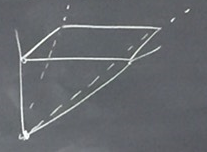
\includegraphics[width=0.5\textwidth]{pic/lec02pic01}
\end{figure}
\end{Eg}
\begin{Remark}
\begin{itemize}
\item $\sigma$ is a face of $\sigma$
\item the smallest face is
\begin{equation*}
\sigma\cap(-\sigma)(=\text{lineality space})
\end{equation*}
\item a face $\tau\leq\sigma$($\leq$ means a face of) is also a polyhedral cone. if $\sigma=\text{vcone}(A_1,\dots, A_n)$ and $u\in\sigma^{\vee}$, then $\tau=\text{vcone}(\{A_i:u\cdot A_i=0\})$.[\#o6 in hand out\#1:columns are gens of $\sigma$, rows are gens of $\sigma^{\vee}$, can figure out all faces($u_i^Tv_j=0$ in entry $(i,j)$)]
\end{itemize}
\end{Remark}

%---- Lecture 03 on Jan. 29th ---------
\newpage
\section{Lecture 03}

\begin{Def}
Let $\sigma \subseteq V$ be a polyhedral cone.
The following are equivalent:
\begin{enumerate}
\item $\sigma \cap (-\sigma) = \{0\}$
\item $\sigma$ contains no non-zero subspace
\item there exists $u \in \sigma^\vee$ such that $\sigma \cap u^\perp = \{0\}$
\item $\dim V = \dim \sigma^\vee$.
\end{enumerate}
If $\sigma$ satisfies the above than it is \emph{strongly convex} or \emph{pointed}.
\end{Def}

\begin{Def}
A \emph{face} of $\sigma$ is a subset $\tau \subseteq \sigma$ of the form $\tau = \sigma \cap u^\perp$ where $u \in \sigma^\vee$.
\end{Def}

Recall that if $\sigma$ is a polyhedral cone than $\mathrm{rel int}(\sigma)$ is the interior of $\sigma \subseteq(\mathrm{span}(\sigma))$ (except $\mathrm{rel int}(0) = 0$).
If $\sigma = \mathrm{vcone}(v_1, \dots, v_r)$ then $\mathrm{rel int}(\sigma) = \{\alpha_1v_1 + \dots + \alpha_rv_r : \alpha_i > 0\}$.

For the following facts let $\sigma = \mathrm{vcone}(v_1, \dots, v_r)$ and $\sigma^\vee = \mathrm{vcone}(u_1, \dots, u_s)$ be irredundant.

\begin{Fact}
Let $\tau_i = \sigma \cap u_i^\perp \subseteq \sigma$.
Then $\tau$ is a facet of $\sigma$.
\end{Fact}

\begin{Fact}
If $\mu = \mathrm{vcone}(u_{i1}, \dots, u_{il})$ is a face of $\sigma^\vee$ and $u \in \mathrm{rel int}(\mu)$ then
\[
\sigma \cap u^\perp = \bigcap_{j=1}^l(\sigma \cap u_{ij}^\perp) = \bigcap_{j=1}^l \tau_j.
\]
\end{Fact}

\begin{proof}
Since $u \in \mathrm{rel int}\mu)$ we have $u = \alpha_iu_{i1} + \dots + \alpha_lu_{il}$ where each $\alpha_j > 0$.
Let $v \in \sigma$.
Then $v \in \sigma \cap u^\perp$ if and only if $\langle u, v \rangle = 0$, which happens if and only if $\alpha_i\langle u_{i1}, v \rangle + \dots + \alpha_l\langle u_{il}, v \rangle = 0$.
But since $v \in \sigma$ we know $\langle u_j, v \rangle \le 0$ for all $u_j$, so this happens if and only if $\langle u_{ij}, v \rangle = 0$ for all $u_{ij}$.
This is equivalent to $v \in \bigcap_{j=1}^l \tau_{ij}$.
\end{proof}

\begin{Fact}
There is an order reversing bijection $\{\text{faces of $\sigma$}\} \to \{\text{faces of $\sigma^\vee$}\}$ given by $\tau \mapsto \sigma^\vee \cap \tau^\perp$ and (in reverse) $\tau^\star \mapsto \sigma \cap (\tau^\star)^\perp$.
For two elements in this bijection we have $\dim \tau + \dim \tau^\star = \dim V$.
\end{Fact}

\begin{Eg}
See the example from handout 1, where $\dim \sigma = 4$.
\end{Eg}

\begin{Def}
If $\sigma \subseteq V = \mathbb{R}^n$ and $\sigma$ is generated by vectors in $\mathbb{Q}^n$ (or equivalently $\mathbb{Z}^n$) we call $\sigma$ a \emph{rational} polyhedral cone.
\end{Def}

[NOTATION YOU DON'T WANT TO FORGET]

Let $M$ be a lattice (a finite abelian group with no torsion), so $M = \mathbb{Z}^n$ for some $n$.
We have
\[
M \subseteq M_{\mathbb{Q}} \subseteq M_{\mathbb{R}}
\]
where $M_k = M \otimes_{\mathbb{Z}} k$ so that $M = \mathbb{Z}^n$, $M_{\mathbb{Q}} = \mathbb{Q}^n$, and $M_{\mathbb{R}} = \mathbb{R}^n$.
Let $N$ be the dual lattice (so $N = \Hom(M, \mathbb{Z})$).
Choose dual coordinates
\[
e_1, \dots, e_n \quad \text{basis of $M$}
\]
\[
e_1^\star, \dots, e_n^\star \quad \text{dual basis of $N$}
\]
and define similarly $N \subseteq N_{\mathbb{Q}} \subseteq N_{\mathbb{R}}$.
Then $N_{\mathbb{Q}} = M_{\mathbb{Q}}^\star$ are dual vector spaces.
We will often use the notation ``$\sigma$ is a cone in $N$" to mean that $\sigma$ is a rational polyhedral cone in $N_{\mathbb{R}}$ (Fulton also adds to this definition that $\sigma^\vee$ is pointed).

\begin{Def}
If $M$ is a lattice then $S \subseteq M$ is a \emph{semigroup} if
\begin{enumerate}
\item $0 \in S$
\item if $m, m' \in S$ then $m + m' \in S$.
\end{enumerate}
\end{Def}

\begin{Eg}
$\mathbb{Z}^n$, $\mathbb{C}$ under multiplication, and $\mathbb{C}^\star$ are all semigroups.
\end{Eg}

\begin{Eg}
$S \subseteq \mathbb{Z}^2$ given by $S = \left\langle \begin{pmatrix}1\\1\end{pmatrix}, \begin{pmatrix}2\\1\end{pmatrix}, \begin{pmatrix}3\\1\end{pmatrix}, \dots \right\rangle$ is a semigroup that is not finitely generated.
\end{Eg}

\begin{Def}
If $\sigma$ is a cone in $N$ than $S_{\sigma} = \sigma^\vee \cap M$.
\end{Def}

(question: why not $S_\sigma = \sigma \cap N$?)

\begin{Eg}
Let $\sigma = \mathrm{vcone}\left(\begin{pmatrix}-2\\1\end{pmatrix}, \begin{pmatrix}0\\-1\end{pmatrix}\right)$.
Then $S_\sigma = \sigma^\vee \cap M = \left\langle \begin{pmatrix}1\\2\end{pmatrix}, \begin{pmatrix}1\\1\end{pmatrix}, \begin{pmatrix}1\\0\end{pmatrix} \right\rangle$.
\end{Eg}

\begin{Proposition}[Gordon's Lemma]
If $\sigma$ is a cone in $N$ then $S_\sigma$ is a finitely generated semigroup.
\end{Proposition}

\begin{proof}
Let $\sigma = \mathrm{vcone}(v_1, \dots, v_s)$ and let $K = \{\alpha_1v_1 + \dots + \alpha_sv_s : 0 \le \alpha_i < 1\}$.
Note that $K$ is bounded so $K \cap M$ is finite.
Clearly, $\sigma^\vee \cap M$ is generated by $v_1, \dots, v_s$ and $K \cap M$.
\end{proof}

\begin{Def}
Let $\sigma$ be a pointed cone in $N$.
Then $m \in \sigma^\vee \cap M = S_\sigma$ is called \emph{irreducible} if $m = m' + m''$ for $m', m'' \in S_\sigma$ means $m' = 0$ or $m'' = 0$.
\end{Def}

\begin{Proposition}
Let $H = \{m \in S_\sigma : \text{$m$ is irreducible}\}$.
Then
\begin{enumerate}
\item $H$ is finite
\item $H$ generates $S_\sigma$
\item every generating set of $S_\sigma$ contains $H$.
\end{enumerate}
\end{Proposition}

The set $H$ from the above proposition is the Hilbert basis of $S_\sigma$.

%---- Lecture 04 on Feb 5 ---------
\newpage
\section{Lecture 04}

Let $\sigma$ be a cone in $N$ (i.e., $\sigma$ is a rational, polyhedral, convex cone in $N_\mathbb{R}$).
Often $\sigma$ is pointed.
Recall that $S_\sigma = \sigma^\vee \cap M \subseteq M$ ($= \mathbb{Z}^n$) is a finitely generated semigroup by its Hilbert basis.

\begin{Def}
Let $A_\sigma = \CC[S_\sigma] = \CC[\sigma^\vee \cap M]$.
This is the $\CC$-algebra such that
\begin{enumerate}
\item $\{t^m : m \in S_\sigma\}$ is a $\CC$-basis for $A_\sigma$
\item $t^{m_1} \cdot t^{m_2} = t^{m_1 + m_2}$
\end{enumerate}
\end{Def}

\begin{Def}
$X_\sigma = \Spec A_\sigma$ is the \emph{affine toric variety} associated to $\sigma$.
\end{Def}

We want to understand:
\begin{itemize}
\item examples
\item ideal
\item points
\item tori and torus action
\item tangent space and singularities
\item toric morphisms.
\end{itemize}

Note that if $\sigma^\vee \cap M = \langle m_1, \dots, m_r \rangle$ then $A_\sigma$ is generated by $\{t^{m_1}, \dots, t^{m_r}\}$.
In particular, $A_\sigma$ is Noetherian.
We have an exact sequence
\[
0 \to \ker \phi \to \CC[x_1, \dots, x_r] \overset{\phi}{\to} A_\sigma \to 0
\]
where $\phi: x_i \mapsto t^{m_i}$.
Then defining $I_\sigma = \ker \phi$ gives that $A_\sigma = \CC[x_1, \dots, x_r]/I_\sigma$.
Thus $X_\sigma = V(I_\sigma) \subseteq \CC^r$ is an affine variety.

\begin{Eg}
Let $\sigma = \mathrm{vcone}\left(\begin{pmatrix}-1\\0\end{pmatrix}, \begin{pmatrix}0\\-1\end{pmatrix}\right)$.

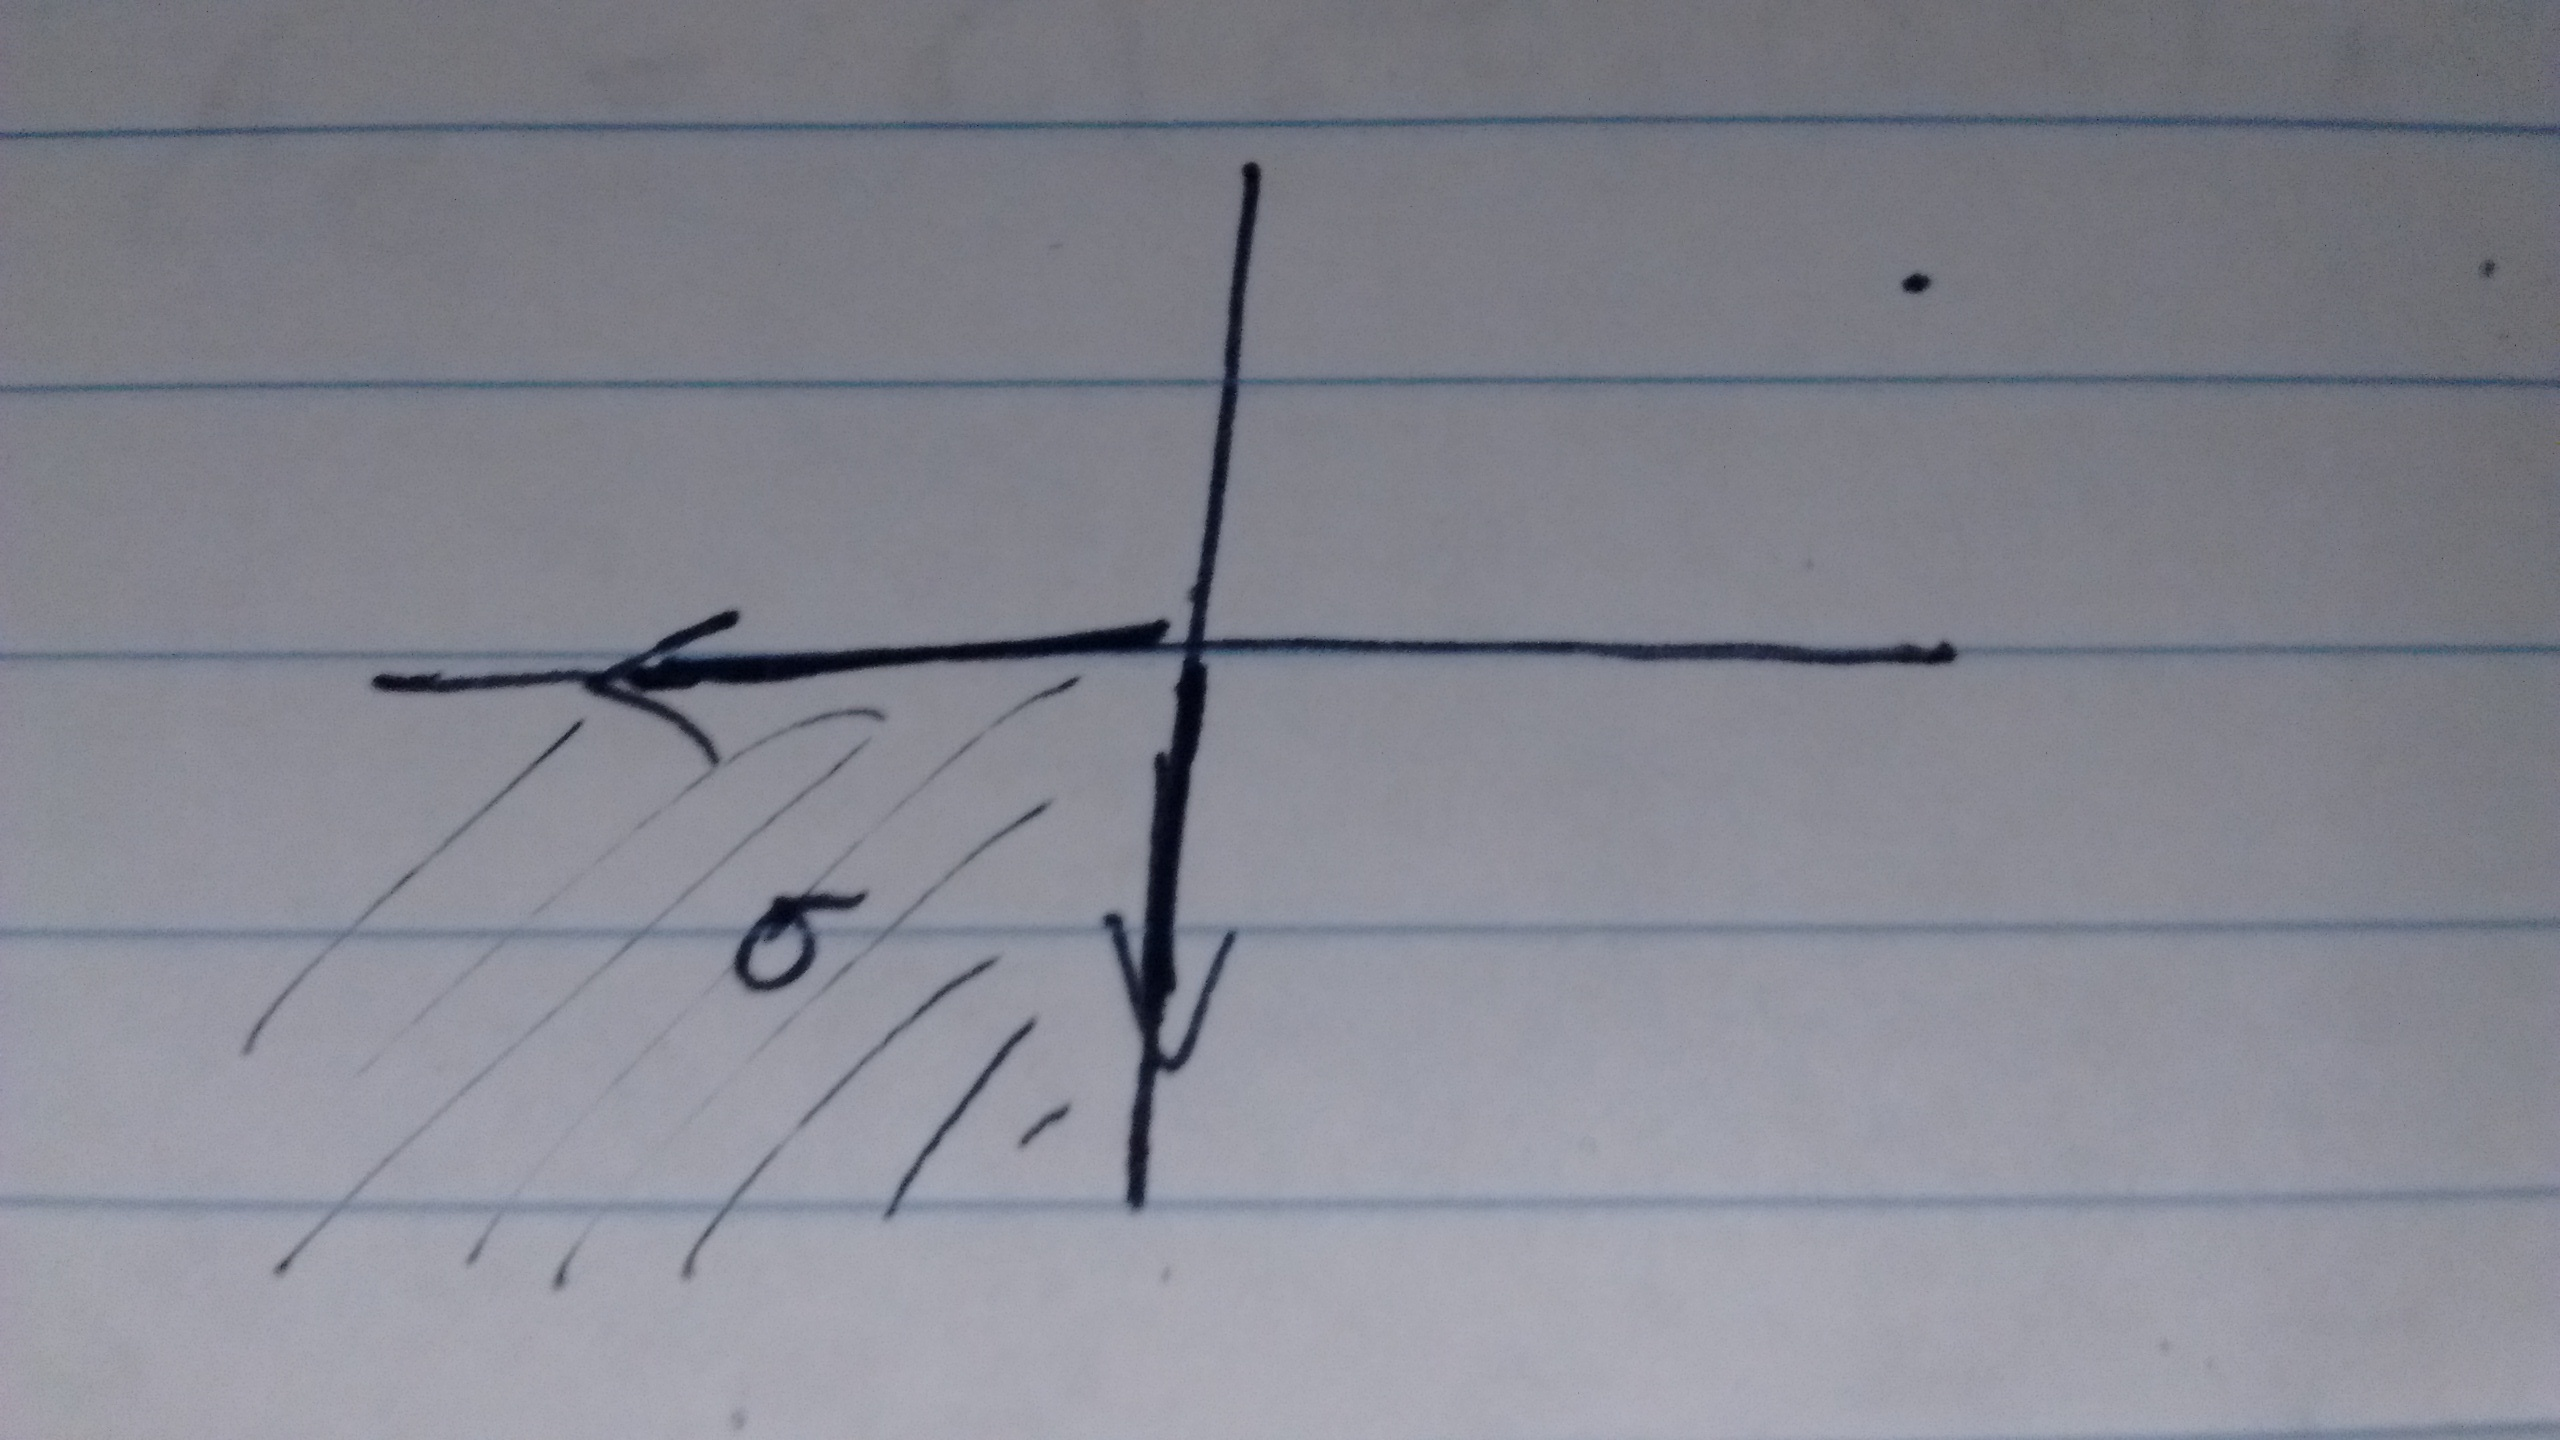
\includegraphics[width=0.3\textwidth]{pic/lec04-pic1}
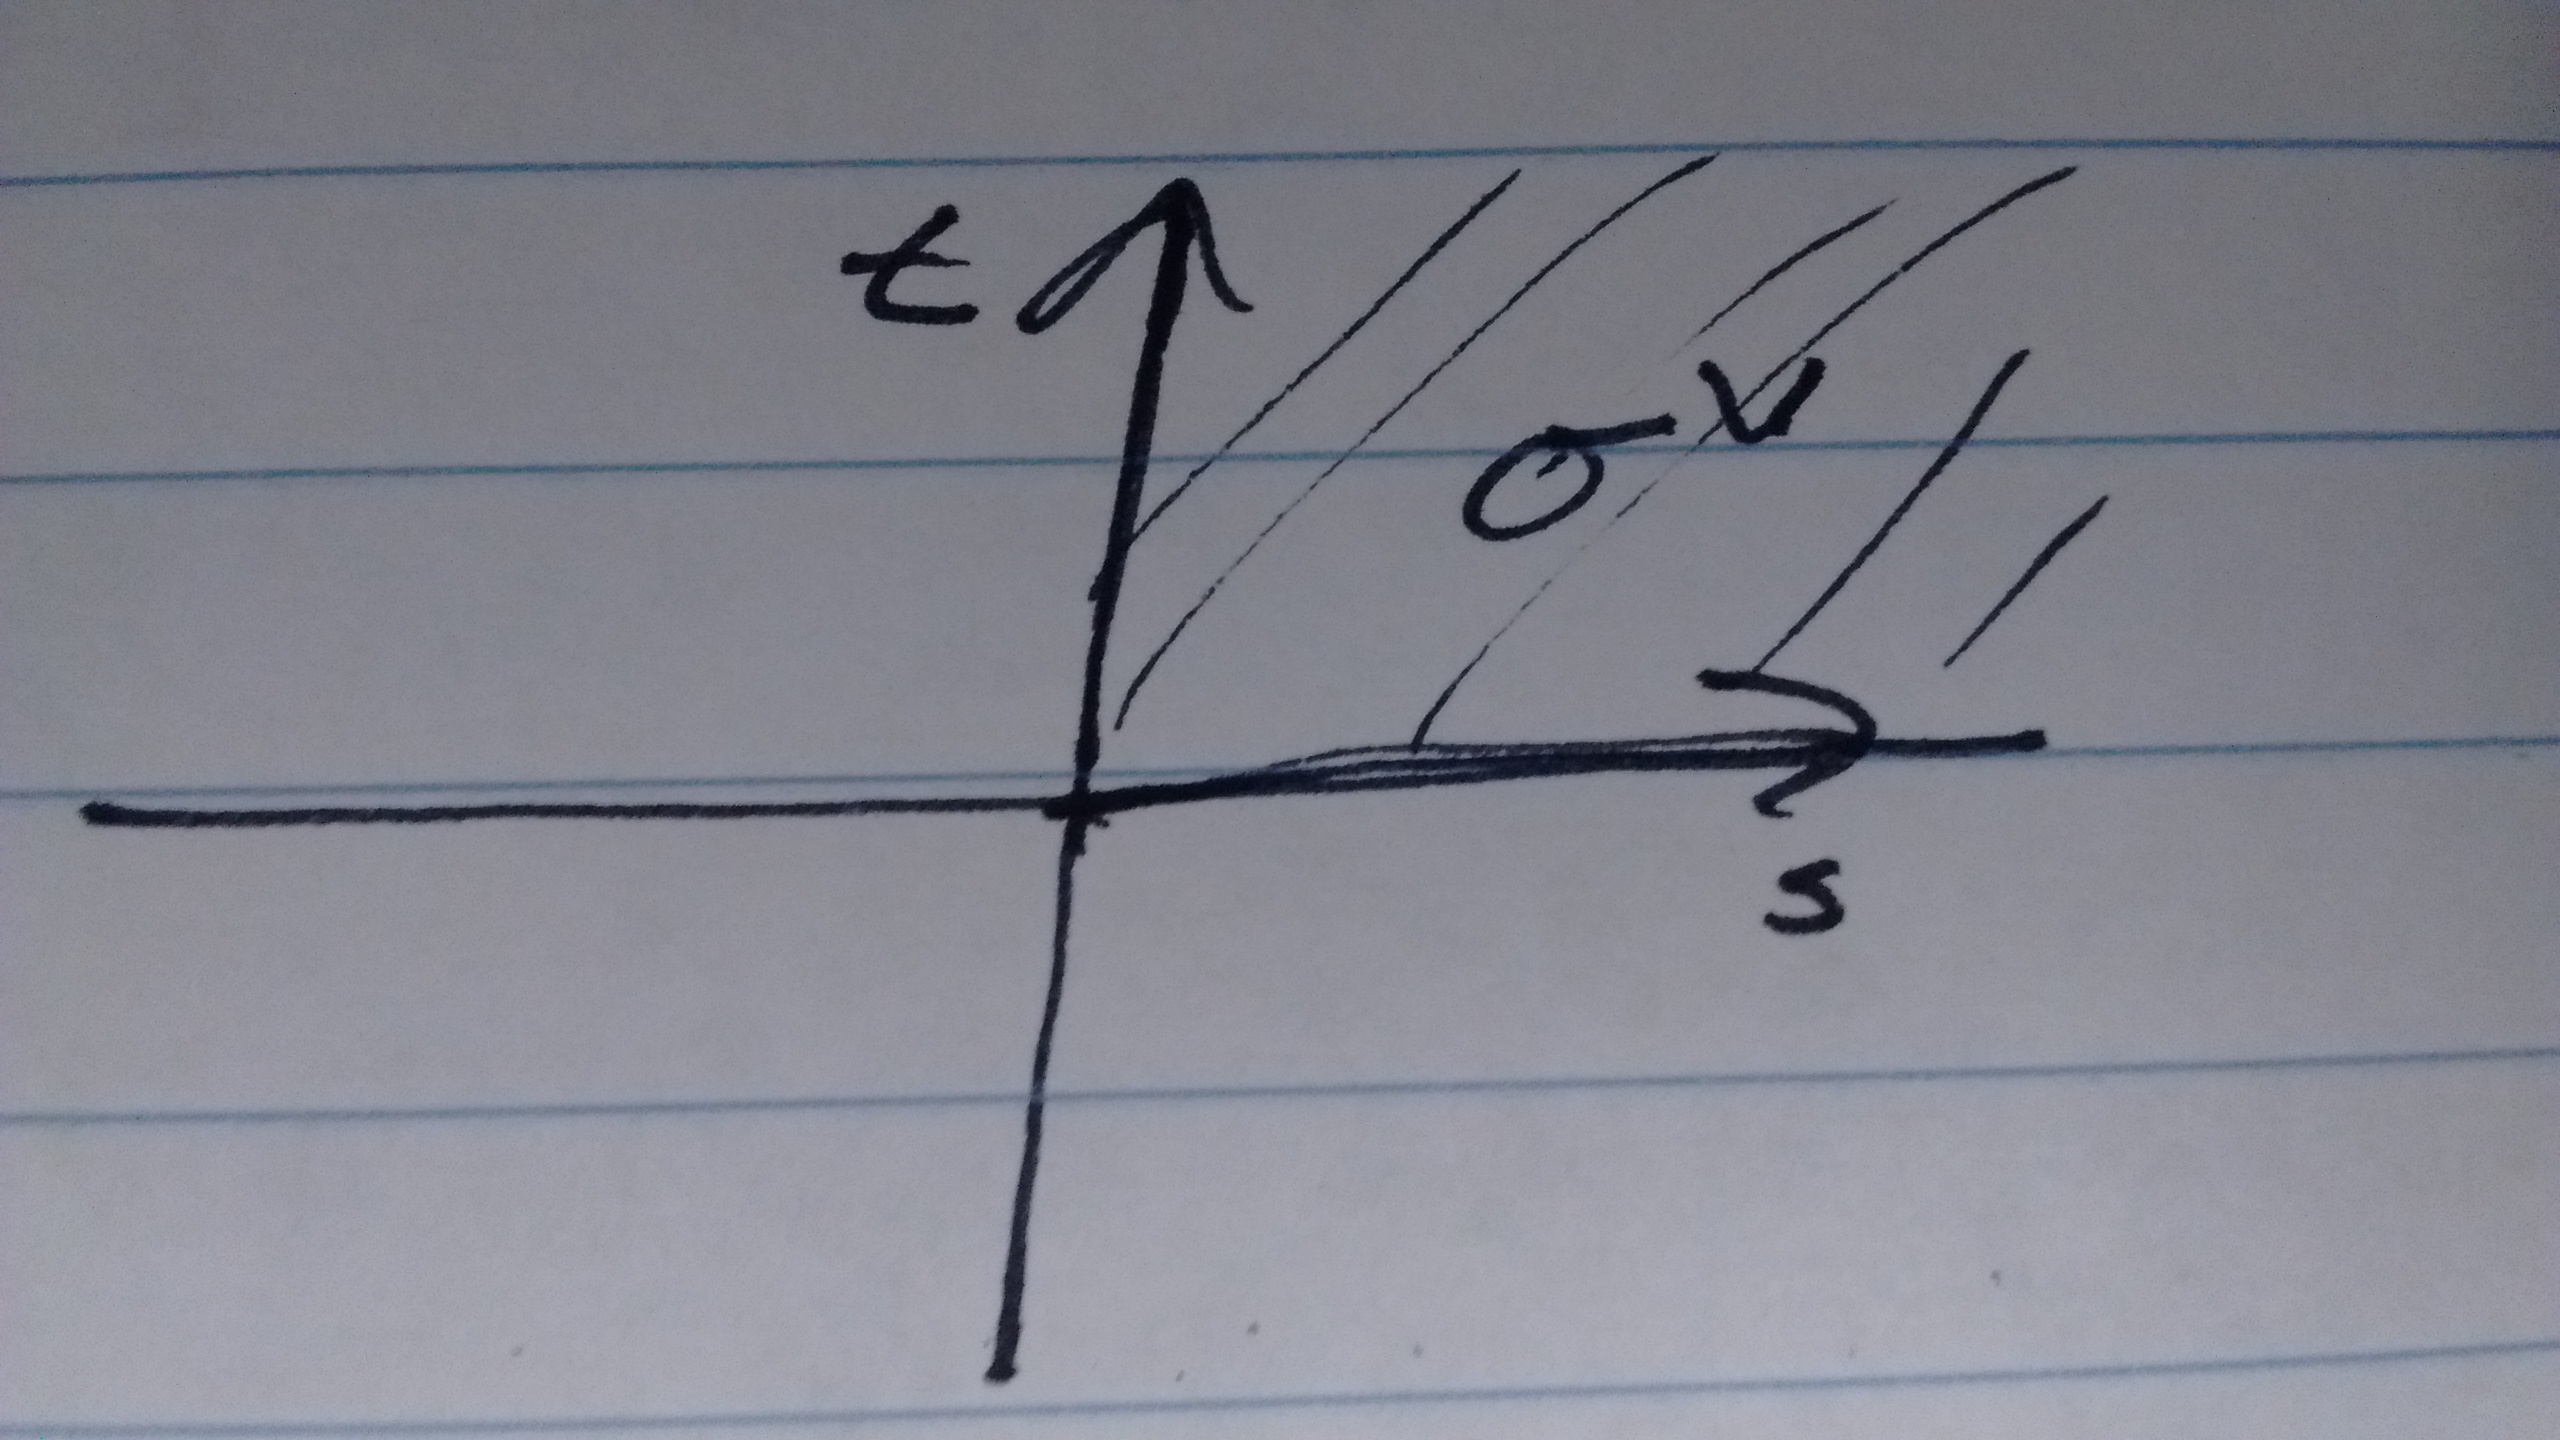
\includegraphics[width=0.3\textwidth]{pic/lec04-pic2}

Then $A_\sigma = \CC[s, t]$ and $X_\sigma = \CC^2$.
\end{Eg}

\begin{Eg}
If $\sigma = \mathrm{vcone}(-I_n) \subseteq \RR^n$ then $X_\sigma = \CC^n$.
If $\sigma = \mathrm{vcone}(I_n)$ then $X_\sigma = \CC^n$ but with different coordinates.
\end{Eg}

\begin{Eg}
Let $\sigma = \{0\}$ in $N = \ZZ^2$.
Then $\sigma^\vee = M_\RR$, $S_\sigma$ is all lattice points, and $A_\sigma = \CC[s,t,s^{-1},t^{-1}] = \CC[s, t]_{st}$.
This gives $X_\sigma = (\CC^\star)^2$, which is the algebraic torus $T$.
\end{Eg}

\begin{Eg}
Let $\sigma = \{0\}$ in $N = \ZZ^n$.
Then $\sigma^\vee = M_\RR$, $S_\sigma$ is all lattice points, and $A_\sigma = \CC[t_1^{\pm 1}, \dots, t_n^{\pm 1}]$.
This gives $X_\sigma = (\CC^\star)^n$, which is often denoted $T_n$.
\end{Eg}

\begin{Eg}
Let $\sigma = \mathrm{vcone}\left(\begin{pmatrix}-1\\2\end{pmatrix}, \begin{pmatrix}0\\-1\end{pmatrix}\right)$.
Then $\sigma^\vee = \mathrm{vcone}\left(\begin{pmatrix}2\\1\end{pmatrix}, \begin{pmatrix}1\\0\end{pmatrix}\right)$.

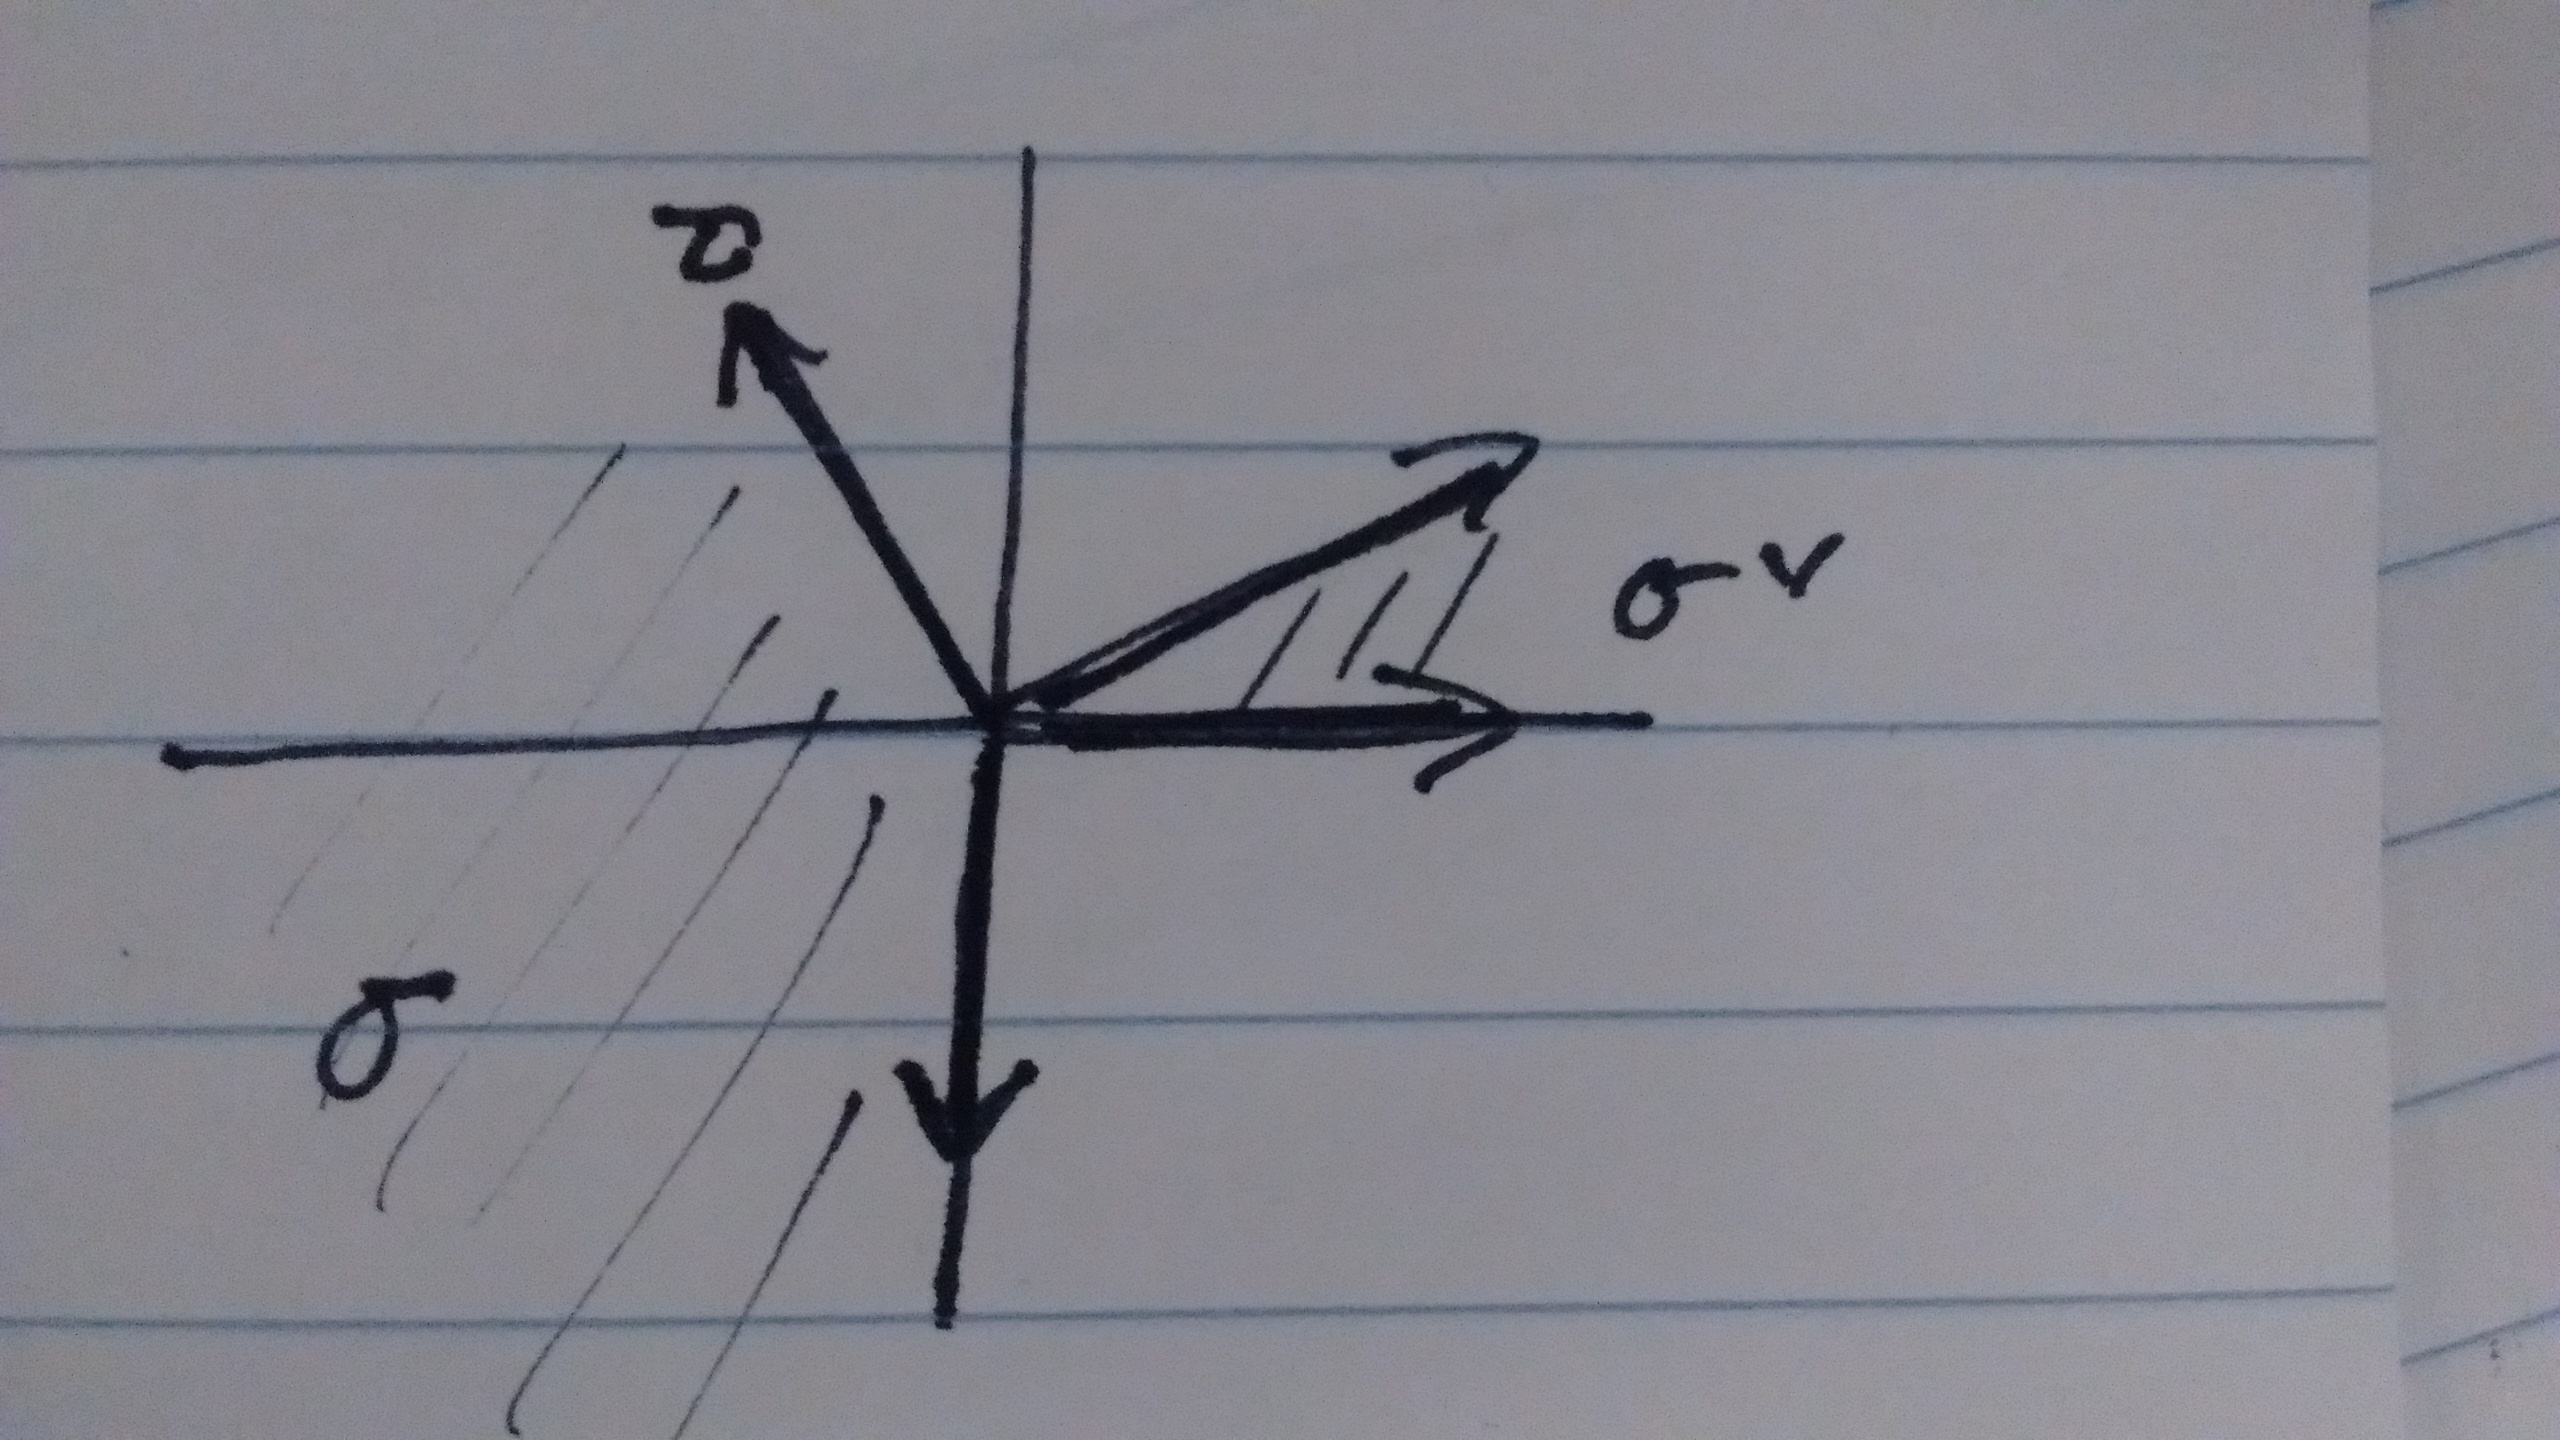
\includegraphics[width=0.3\textwidth]{pic/lec04-pic3}

We have $A_\sigma = \CC[s, s^2t] = \CC[u, v]$ and $X_\sigma = \CC^2$.

Now let $\tau = \mathrm{vcone}\left(\begin{pmatrix}-1\\2\end{pmatrix}\right)$ so $\tau^\vee = \mathrm{vcone}\left(\begin{pmatrix}2\\1\end{pmatrix}, \begin{pmatrix}-2\\1\end{pmatrix}, \begin{pmatrix}1\\0\end{pmatrix}\right)$.
Then $A_\tau = \CC[s^2t, (s^2t)^{-1}, s] = (A_\sigma)_{s^2t}$ and $X_\tau = \CC \times \CC^\star \hookrightarrow X_\sigma$ as an open set.
\end{Eg}

Exercise: If $\sigma$ is not pointed, what is $A_\sigma$ and $X_\sigma$?

As before, let $\sigma^\vee \cap M = \langle m_1, \dots, m_r \rangle$ and consider the exact sequence
\[
0 \to I_\sigma \to \CC[x_1, \dots, x_r] \overset{\phi}{\to} A_\sigma \to 0.
\]
Note that $A_\sigma = \CC[\sigma^\vee \cap M] \subseteq \CC[M] = \CC[t_1^{\pm 1}, \dots, t_n^{\pm 1}]$ and $\CC[t_1^{\pm 1}, \dots, t_n^{\pm 1}]$ is a domain.
Thus $A_\sigma$ is a domain, $I_\sigma$ is prime, and $X_\sigma$ is irreducible.


%---- Lecture 05 on Feb 7 ---------
\newpage
\section{Lecture 5}

Recall some notation and observations from last time:
\begin{align*}
A_\sigma := \CC[\sigma^\vee \cap M]
X_\sigma = \Spec A_\sigma = \bb{V}(I_\sigma) \subseteq \CC^r
\end{align*}
if $\sigma^\vee \cap M = \langle m_1, ..., m_r \rangle$ then the natural projection $\varphi: x_i \mapsto m_i$ forms an exact sequence
\begin{center}
	\begin{tikzcd}
		0 \arrow[r] & I_\sigma \arrow[r] & {\CC[x_1,...,x_r]} \arrow[r, "\varphi"] & A_\sigma \arrow[r] & 0.
	\end{tikzcd}
\end{center}

Recall from last time that $I_\sigma$ is a prime ideal, so that $X_\sigma$ is an irreducible (reduced) variety. What is $I_\sigma$?

\begin{Proposition}
$I_\sigma$ is generated by $\langle x_1^{\alpha_1} \cdots x_r^{\alpha_r} - x_1^{\beta_1} \cdots x_r^{\beta_r} : \forall i (\alpha_i, \beta_i \geq 0, \sum_i \alpha_i m_i = \sum_i \beta_i m_i) \rangle $.
\end{Proposition}
\begin{proof}

($\supseteq$) $\varphi(x_1^{\alpha_1} \cdots x_r^{\alpha_r}) = t^{\sum_i \alpha_i m_i}$ and $\varphi(x_1^{\beta_1} \cdots x_r^{\beta_r}) = t^{\sum_i \beta_i m_i}$

($\subseteq$) Note that $x^\alpha - x^\beta \in I_\sigma \iff \sum_i \alpha_i m_i = \sum_i \beta_i m_i$. Note as well that if $J := \langle t^{m_1} - x_1, ..., t^{m_r} - x_r\rangle \subseteq \CC[t_1, ..., t_n x_1, ..., x_r]$ (where $M = \ZZ^n$ is generated by $e_1, ..., e_n$, and we let $t_i := t^{e_i}$) then $I_\sigma = J \cap \CC[x_1, ..., x_r]$.

In order to see this, recall the theory of Groebner bases. Choose the lexicographic monomial order $t_1 > t_2 > ... > x_r$. Let $G$ be the Groebner basis of $J = \{g_1, ..., g_N\}$ in this order. Then $J \cap \CC[x_1, ..., x_r]$ is generated by the $\{g_i : g_i \in \CC[x_1, ..., x_r]$. It is easy to see that $G$ is generated by binomials.
\end{proof}
\paragraph{Products (exercise)}
Suppose $\sigma$ is a cone in $N$, and $\sigma'$ is a cone in $N'$. Then 
\begin{enumerate}
	\item $\sigma \times \sigma'$ is a cone in $N \oplus N'$
	\item $(\sigma \times \sigma')^\vee =$ ???
	\item $A_{\sigma \times \sigma'} =$ ???
	\item Show that $X_{\sigma \times \sigma'} \simeq X_\sigma \times X_{\sigma'}$ ( $= X_\sigma \times_{\Spec \CC} X_{\sigma'}$ )
\end{enumerate}

\begin{Eg}
Let

$\sigma = 0 \subset N = \ZZ^r$

$\sigma' = \langle e_1, ..., e_s \rangle \subseteq N' = \ZZ^s$ ($\sigma' = N'_\RR$)

then $X_\sigma \times X_{\sigma'} = (\CC*)^r \times \CC^s$.
\end{Eg}

The plan for this session is to cover some local properties of $X_\sigma$. This includes \textit{points}, the \textit{zariski tangent space}, the \textit{torus action} and the \textit{cone-orbit correspondence} in the affine case.


\paragraph{Points on $X_\sigma$}
If $X$ is a variety (or scheme) then a (closed) point of $X$ is ``really'' a morphism  $\Spec \CC \to X$ (understanding $\Spec \CC$ as a point).

Unraveling this, we have a map $\varphi: \Spec \CC \to \Spec \CC[\sigma^\vee \cap M]$, so that the data of $\varphi$ is corresponds one to one with the data of a map $\varphi^\#: \CC[\sigma^\vee \cap M] \to \CC$, an \textit{evaluation map}. Such a map corresponds one to one with a semigroup homomorphism $\rho: \sigma^\vee \cap M \to \CC^\times$ (i.e. $\rho(m_1 + m_2) = \rho(m_1) \rho(m_2)$ whenever $m_1$ and $m_2$ are in $\sigma^\vee \cap M$, and $\rho(id) = 1$).

In other words, we have a correspondence 
\begin{center}
	\begin{tikzcd}
		\text{points of } X_\sigma \arrow[rr] &  & {\Hom_{\text{semigroup}} (\sigma^\vee \cap M, \CC)} \arrow[ll, "1 \text{ to } 1"'].
	\end{tikzcd}
\end{center}

\begin{Def}[Distinguished point]
$p_\sigma \in X_\sigma$ is the point corresponding to 
\begin{align*}
\sigma^\vee \cap M &\to \CC \\
m &\mapsto \begin{cases}
1 \text{ if } m \in \sigma^\perp \\
0 \text{ if } m \not \in \sigma^\perp
\end{cases}
\end{align*}
\end{Def}
Note that if $\sigma$ is full dimensional then this map sends $m$ to $1$ if and only if $m = 0$. This is a semigroup homomorphism since if $m_1, m_2 \in \sigma^\vee \cap M$ then $m_1 + m_2 \in \sigma^\perp \iff m_1, m_2 \in \sigma^\perp$.

\begin{Proposition}
	Let $\tau \leq sigma$ (i.e. $\tau$ is a face of $\sigma$). Let $u \in \sigma^\vee \cap M$ s.t. $\tau = \sigma \cap u^\perp$. Then $S_\tau = S_\sigma + \ZZ_{\geq 0} \cdot (-u)$. 
\end{Proposition}
\begin{proof}
Exercise.
\end{proof}

\begin{Def}[Principal affine open sets]
If $X$ is an affine variety, and $f \in A(X)$, then $U_f := X \setminus V(f) \subset X$ is called a \textbf{ principal (affine) or basic open set of $V$}.
\end{Def}

\begin{Corollary}
If $\tau \leq \sigma$, and $u$ is as above, then $A_\tau = (A_\sigma)_{t^{u}}$ and so $X_\tau \subseteq X_\sigma$ is a principal open set. 
\end{Corollary}
Note: If $\tau \leq \sigma$ is a face, we have $p_\tau \in X_\tau \subset X_\sigma$. In other words, we have distinguished points $p_\tau \in X_\sigma$ for all faces $\tau$ of $\sigma$.

\paragraph{Example}
Consider the cone $\sigma$ pictured below in red:

\begin{center}
	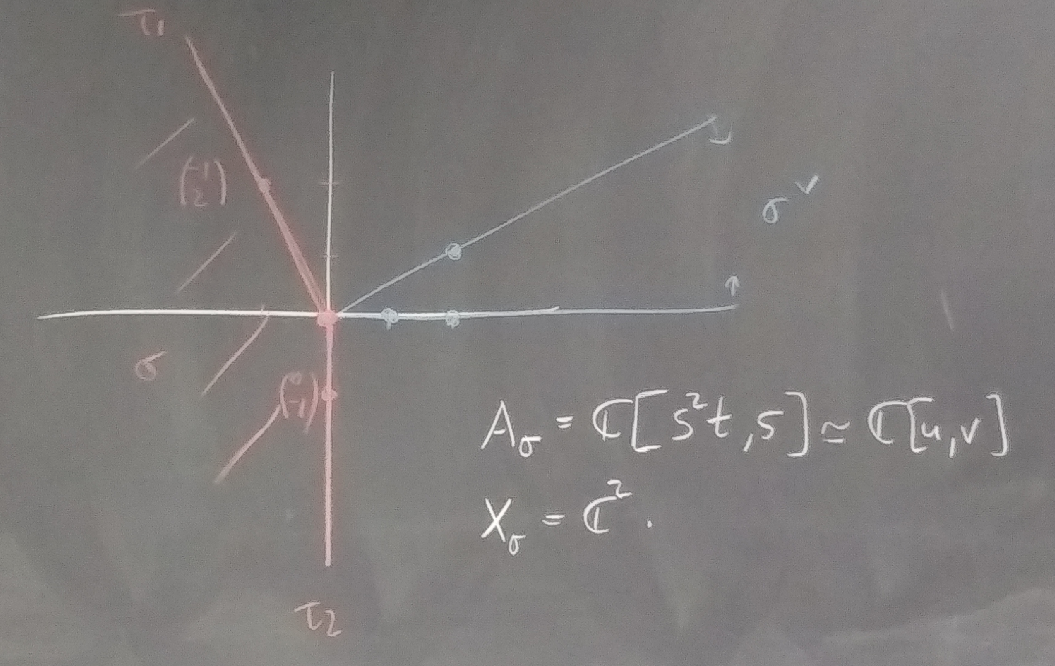
\includegraphics[scale=0.2]{pic/toricvar_feb7_1}
\end{center}

We want to understand the points $p_\sigma, p_{\tau_1}, p_{\tau_2}, p_0$.
\begin{enumerate}
	\item $p_\sigma(m) = \begin{cases}
	1 \text{ if } m = 0 \\
	0 \text{ if } m \neq 0 \\
	\end{cases}$
	
	so that $p_\sigma = (0,0) \in \CC^2_{uv}$.
	\item $p_{\tau_1} = (1,0)$
	\item $p_{\tau_2} = (0,1)$
	\item $p_{0} = (1,1)$
\end{enumerate}
We have inclusions on open sets given by the diagrams:
\begin{center}
	\begin{tikzcd}
		& X_{\tau_1} = \CC^* \times \CC \arrow[rd, hook] &  \\
		(\CC^*)^2 = X_0 \arrow[rd, hook] \arrow[ru, hook] &  & X_\sigma = \CC^2 \\
		& X_{\tau_2} = \CC \times \CC^* \arrow[ru, hook] & 
	\end{tikzcd}
\end{center}

\paragraph{Zariski tangent space / nonsingularity}
Recall: if $X \subseteq \CC^n$ is an affine variety, $A(X) = \CC[x_1, ..., x_n]/I$. If $p \in X$ is a (closed) point: $p = (p_1, ..., p_n) \in X \subseteq \CC^n$, we have an exact sequence 
\begin{center}
	\begin{tikzcd}
		0 \arrow[r] & \mathfrak{m}_p \arrow[r] & {\CC[x_1, ..., x_n]/I} \arrow[r, "ev_p"] & \CC \arrow[r] & 0
	\end{tikzcd}
\end{center}
where $\mathfrak{m}$ denotes the maximal ideal of $p$ in $X$, and $ev_p$ is the evaluation map sending each $x_i$ to $p_i$ (in the language of sheaves, $\mathfrak{m}_p = \mathfrak{m}_{X,p} = \mathcal{O}_{X,p}$).

We define the \textbf{Zariski cotangent space} at the point $p$ as $T^*_{X, p} := \mathfrak{m}_p / \mathfrak{m}_p^2$, a finite dimensional $\CC$-vector space. Similarly, the \textbf{Zariski tangent space} is $T_{X,p} := (\mathfrak{m}_p / \mathfrak{m}_p^2)^*$, the dual vector space.

(Note: A basic fact from any basic reference, for example the first chapter of Hartshorne, states that $\dim_\CC T_{X,p} \geq \dim_p X$, where $\dim_p X$ is the Krull dimension of $\mathcal{O}_{X,p}$. Also, $X$ is nonsingular at $p$ exactly when equality is achieved.) \\

Our situation is the following. We have a pointed cone $\sigma$ in $N$, a corresponding toric variety $X_\sigma$, and a distinguished point $p_\sigma \in X_\sigma$, along with other distinguished points $X_\tau$. The following questions arise:
\begin{enumerate}%[label=(\arabic*)]
	\item How do we identify $T_{X_\sigma, p_\tau}$, or at least its dimension?
	\item How do we study other points of $X_\sigma$?
	\item How do we identify the singular locus, or set of singular points.
\end{enumerate}

\paragraph{Proposition}
\begin{Proposition}
$\dim T_{X_\sigma, p_\sigma} = \mathcal{H}$, where $\mathcal{H}$ is the Hilbert basis of $\sigma^\vee \cap M$.
\end{Proposition}
\begin{proof}
Recall that $p_\sigma(m) = \begin{cases}
0, m \neq 0 \\
1, m = 0 
\end{cases}$. What is $\mathfrak{m}_{p_\sigma}$? 

We know that $A_\sigma = \bigoplus_{m \in \sigma^\vee \cap M} \CC \cdot t^m$ so $\mathfrak{m}_p = \bigoplus_{m \neq 0} \CC \cdot t^m \subset A_\sigma$. We also have $\mathfrak{m}_p^2 = \bigoplus_{m \text{ not irreducible}} \CC \cdot t^m$, so that 
\begin{align*}
\mathfrak{m}_p / \mathfrak{m}_p^2 = \sum_{m \in \mathcal{H}} \CC \cdot t^m \implies \dim \mathfrak{m}_p / \mathfrak{m}_p^2 =  | \mathcal{H} | 
\end{align*}
and the result follows.
\end{proof}

\begin{Remark}
	Assume $\sigma$ is a pointed cone in $N$. What is $\dim X_\sigma$? We can get a torus $T = (\CC^*)^n \subseteq X_\sigma$ an inclusion of an open subset, where $n$ is the rank of $N$. So the field of rational functions on $X_\sigma$ satisfies $K(X_\sigma) = K((\CC^*)^n) = \CC(t_1, ..., t_n)$, and this is the dimension of $X$. 
\end{Remark}
Suppose now $X_\sigma$ is smooth, that is, nonsingular, and once again that $\sigma$ is a pointed cone of maximal dimension. Then $\dim T_{X, p_\sigma} = \dim X = n$, so the Hilbert basis $\mathcal{H}$ of $\sigma^\vee \cap M$ satisfies $|\mathcal{H}| = n$. Because $X$ has maximal dimension, it has at least $n$ extremal rays. But $|\mathcal{H}| \geq \# \textit{ extremal rays } \geq n$, so that the number of extremal rays is exactly $n$.


%---- Lecture 06 on Feb 12 ---------
\newpage
\section{Lecture 6}

The general topics covered in this session are
\begin{itemize}
\item nonsingular affine toric varieties
\item torus, the torus action on $X_\sigma$
\item orbit-cone correspondence 
\end{itemize}

\paragraph{From last time:}
Recall that the dimension of the tangent space satisfies
\begin{align*}
	\dim T_{X_\sigma, p_\sigma} = | \mathcal{H} |
\end{align*}
where $\mathcal{H}$ is the Hilbert basis of $\sigma^\vee$ (with $\sigma$ a maximal dimension, pointed cone). Note that we use \textit{smooth} to mean nonsingular, that is, without singular points. 

Suppose that $X_\sigma$ is smooth, with $\sigma$ a pointed cone in $N$. Assume that $\sigma$ has maximal dimension $n = \dim N$. Then each extremal ray of $\sigma^\vee$ contains exactly one element of $\mathcal{H}$.	But $|\mathcal{H}| = n$, therefore the number of extremal rasys is at most $n$. Since $\sigma^\vee$ spans $M_\RR$, we have that the number of extremal rays is exactly $n$.  \\

The Hilbert basis $|\mathcal{H}|$ generates $\sigma^\vee \cap M$ as a semigroup, and $M$ as a group. Therefore, the extremal rays (that is, the first element in each ray in $M$) form a $\ZZ$-basis of $M$. Let $m_1, ..., m_n$ be this basis. Then $\CC[\sigma^\vee \cap M] = \CC[x_1, ..., x_n]$ so that $X_\sigma = \CC^n$. In other words, $X_\sigma$ is smooth if and only if $X_\sigma \simeq \CC^n$.

\begin{Def}
A subsemigroup $S \subseteq M$ is \underline{saturated} (in $M$) if whenever $m \in M$ and $pm \in S$ for some $p \in \ZZ_{> 0}$ then $m \in S$.
\end{Def}


\begin{Lemma}\label{lemma1}
	If $\sigma$ is a cone in $N$ then $S := \sigma \cap N$ is saturated. (In particular, $S_\sigma = \sigma^\vee \cap M$ is also saturated.)
\end{Lemma}
\begin{proof}
	If $pm \in S = \sigma \cap N$, with $m \in N$, then $pm \in \sigma$ implies that $m \in \sigma$. Therefore we get that $m \in \sigma \cap N$.
\end{proof}

\begin{Lemma}\label{lemma2}
If $\sigma$ is a cone in $N$, let $N_\sigma$ be the lattice spanned by $\sigma \cap N$. Then $N/N_\sigma$ is a lattice. 
\end{Lemma}
\begin{proof}
	Suppose not, so that there exist $p \geq 1$ and $v \in N$ not in $N_\sigma$ such that $pv \in N_\sigma$. However, $N_\sigma \subseteq N$ is saturated because $N_\sigma = \text{span}(\sigma) \cap N$, reaching a contradiction.
\end{proof}

\begin{Theorem}
	Let $\sigma$ be a pointed cone in $N$, $\dim \text{span}(\sigma) = k$. The following are equivalent:
	\begin{enumerate}
		\item $X_\sigma$ is smooth.
		\item $X_\sigma = \CC^k \times (\CC^*)^{n-k}$.
		\item $\sigma$ is generated by a part of a basis of $N$.
	\end{enumerate}
\end{Theorem}

\begin{proof}
	If $k = n$, then we are done by our previous observations. Suppose then that $k < n$. Let $N_\sigma \subseteq N$ be the lattice generated by $\sigma \cap N$ (note that rank $N_\sigma = k$). By Lemma \ref{lemma2}, $N/N_\sigma$ is a lattice. In other words, one can choose a lattice $N'' \subseteq N$ of rank $n-k$ such that 
	\begin{align*}
	N = N_\sigma \oplus N'' (= N' \oplus N'').
	\end{align*}
	Let $\sigma = \sigma' \oplus 0$ in $N' \oplus N''$ (with $N' := N_\sigma)$. Then $\sigma^\vee = (\sigma')^\vee \oplus M''$, with $M'' := \Hom_\ZZ(N'', \ZZ)$. Writing $M = M' \oplus M''$, we therefore get $\sigma^\vee \cap M = ((\sigma')^\vee \cap M') \oplus M''$, so that 
	\begin{align*}
	X_\sigma = X_{\sigma'} \times (\CC^*)^{n-k}
	\end{align*}
	with $\sigma'$ max dimensional in $M'_{\RR}$ (that is, of dimension $k$). Note that $X_\sigma$ is smooth if and only if $X_{\sigma'}$ is smooth, so then $X_{\sigma}$ smooth implies that $X_{\sigma'} \simeq \CC^k$. This proves (a) $\iff$ (b). In this case, we get
	\begin{align*}
	(\sigma')^\vee \cap M' \text{ is generated by a basis of } M' \\
	\iff \sigma' \cap N' \text{ is generated by a basis of } N' \\
	\iff \sigma \text{ is generated by a part of a basis of } N
	\end{align*}
	proving (b) $\iff$ (c) as well.
\end{proof}

\begin{Def}
Let $\sigma$ be a pointed cone in $N = \ZZ^n$. 
\begin{enumerate}
	\item $\sigma$ is called \underline{simplicial} if the number of extremal rays of $\sigma$ is equal to the dimension of $\sigma$ (also call $X_\sigma$ simplicial in this case).
	\item $\sigma$ is \underline{smooth} if $\sigma$ is generated (as semigroup) by a part of a $\ZZ$-basis of $N$.
\end{enumerate}
\end{Def}

\begin{Eg}
Consider the cone $\sigma$ in $N = \ZZ^2$ as in the following image
\begin{center}
	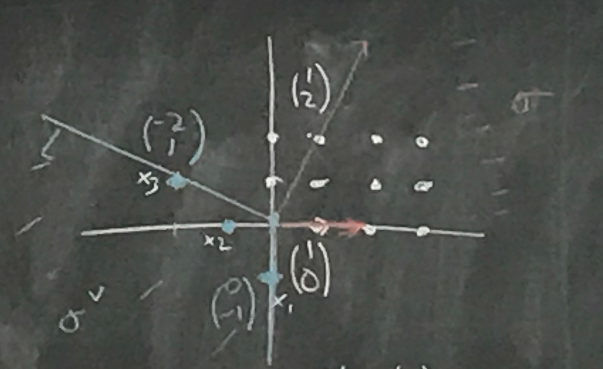
\includegraphics[scale=0.4]{pic/toricvar_feb12_1}.
\end{center}
Note that det$\begin{bmatrix}
1 & 1 \\
0 & 2 
\end{bmatrix} = 2 \neq \pm 1$. We have $|\mathcal{H}_{\sigma^\vee}| = 3$, and $A_\sigma = \CC[x_1, x_2, x_3] / (x_1 x_3 - x_2^2)$. In this case $X_\sigma$ is singular. \underline{Exercise}: Prove $X_\sigma$ is singular at $(0,0,0)$.	
\end{Eg}


\paragraph{Tori, Torus action}
Define, if $N = \ZZ^n$, 
\begin{align*}
	T = T_N := (\CC^*)^n = X_0 = \Spec \CC[M],
\end{align*}
where $0$ denotes the $0$ cone. We can deduce that $T$ is a group, with the operation 
\begin{align*}
	(x_1, ..., x_n)(y_1, ..., y_n) = (x_1 y_1, ... , x_n y_n) \in (\CC^*)^n.
\end{align*}
Consider the distinguished point $(1, ..., 1)$ of $T$. Then the orbit of this point under $T$ is all of $T$. In our previous notation, a point $p = (a_1, ..., a_n) \in (\CC^*)^n$ of $T$ corresponds to the evaluation map $p: M \to \CC^*$ which sends each generator $e_i$ to $a_i$. If $q$ is another point of $T$, then $pq: M \to \CC^*$ satisfies $(pq)(m) = p(m) q(m)$. \\

We wish to define an action of $T$ on $X_\sigma$ by 
\begin{align*}
	T \times X_\sigma &\to X_\sigma \\
	(t,x) &\mapsto t \cdot x.
\end{align*}
when $t: M \to \CC^*$ and $x: \sigma^\vee \cap M \to \CC$ are semigroup homomorphisms, we want the product to also be one, so we define
\begin{align*}
		t \cdot x: \sigma^\vee \cap M &\to \CC \\
	m &\mapsto t(m) x(m).
\end{align*}
and we may check that this is a semigroup homomorphism.

\paragraph{Orbit-cone correspondence}
Consider $X_\sigma$, for $\sigma$ a pointed cone in $N$. 
\begin{enumerate}
\item For $\tau \leq \sigma$ (i.e. a face of $\sigma$) we have that $X_\tau \hookrightarrow X_\sigma$ is a dense open subset. 
\item $X_0 = T \hookrightarrow X_\sigma$ (that is, $X_\sigma$ contains $(\CC^*)^n$).
\item For $\tau \leq \sigma$, we have $p_\tau \in X_\tau \subseteq X_\sigma$.
\end{enumerate}
Define
\begin{enumerate}
\item $\mathcal{O}_\tau := T \cdot p_\tau \subseteq X_\sigma$, the orbit of $p_\tau$.  
\item $V(\tau) := \overline{\mathcal{O}_\tau} \subseteq X_\sigma$, the closure of the orbit.
\item We have a decomposition, into $X_\tau$ and $X_\sigma \setminus X_\tau$.
\end{enumerate}

\begin{Eg}
Let
\begin{align*}
\sigma &= \text{vcone} \begin{bmatrix}
0 & 1 & 1 & 0 \\
0 & 0 & 1 & 1 \\
1 & 1 & 1 & 1 \\
\end{bmatrix} \text{ in } N = \ZZ^3 \\
\sigma^\vee &= \text{vcone} \begin{bmatrix}
0 & 1 & 0 & -1 \\
-1 & 0 & 1 & 0 \\
0 & -1 & -1 & 0 \\
\end{bmatrix} \text{ in } N = \ZZ^3 \text{, labeling the columns } (x_1, ..., x_4) \text{ from left to right } \\
A_\sigma &= \CC[\sigma^\vee \cap M] = \CC[x_1, x_2, x_3, x_4] / \langle x_1 x_3 - x_2 x_4 \rangle
\end{align*}
so that the points of $X_\sigma$ are the quadruples $(x_1, ..., x_4)$ such that $x_1 x_3 = x_2 x_4$. Then $T$ acts as:
\begin{align*}
	(t_1, t_2, t_3) (x_1, x_2, x_3) = (t_2^{-1} x_1, t_1 t_3^{-1} x_2, t_2 t_3^{-1} x_3, t_1^{-1} x_4)
\end{align*}
and this is still in $X_\sigma$. Labeling the faces and edges as in the following picture 
\begin{center}
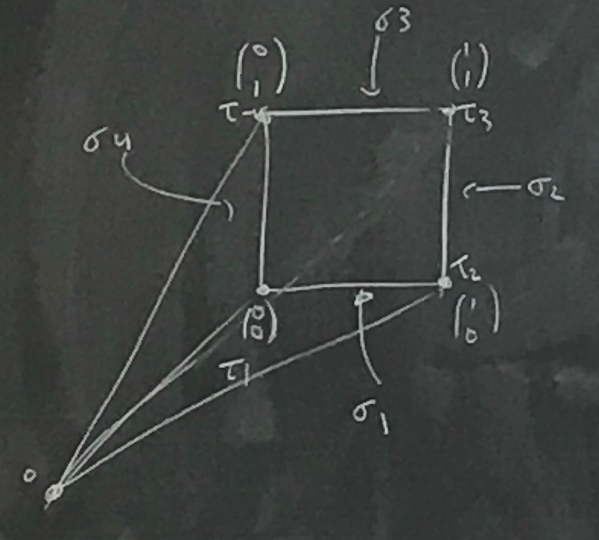
\includegraphics[scale=0.4]{pic/toricvar_feb12_2}.
\end{center}
we may fill out the correspondence in a table (\underline{Exercise}: Fill out the remaining entries in the table):

\begin{center}
\begin{tabular}{|l|l|l|l|l|l|}
\hline
\textbf{$\tau ^*$} & \textbf{$\tau$} & \textbf{$\dim \tau$} & \textbf{$p_\tau \in \CC^4$} & \textbf{$\dim V(\tau)$} & \textbf{$I(V(\tau))$} \\ \hline
$0$ & $\sigma$  & $3$ &  $(0,0,0,0)$ & $0$ & $(x_1, x_2, x_3, x_4)$ \\ \hline
$x_1$ & $\sigma_1$  & $2$ & $(1,0,0,0)$   & $1 = \CC^*$  & $(x_2, x_3, x_4)$  \\ \hline
$x_2$ & $\sigma_2$ &  $2$ & &  &  \\ \hline
$x_3$ & $\sigma_3$ &  $2$ & &  &  \\ \hline
$x_4$ & $\sigma_4$ &  $2$ & &  &  \\ \hline
$x_4 x_1$ & $\tau_1$  & $1$ &  &  &  \\ \hline
$x_1 x_2$ & $\tau_2$ & $1$ &  &  &  \\ \hline
$x_2 x_3$ & $\tau_3$ & $1$ &  &  &  \\ \hline
$x_3 x_4$ & $\tau_4$ & $1$  &  &  &  \\ \hline
$\sigma^\vee$ & $0$  & $0$ & $(1,1,1,1)$  & $3 = T = (\CC^*)^3$  &  \\ \hline
\end{tabular}
\end{center}
\end{Eg}

\newpage
\section{February 14 Lecture}
\subsection{Orbit-cone correspondence}
\begin{figure}[h]
	\centering
	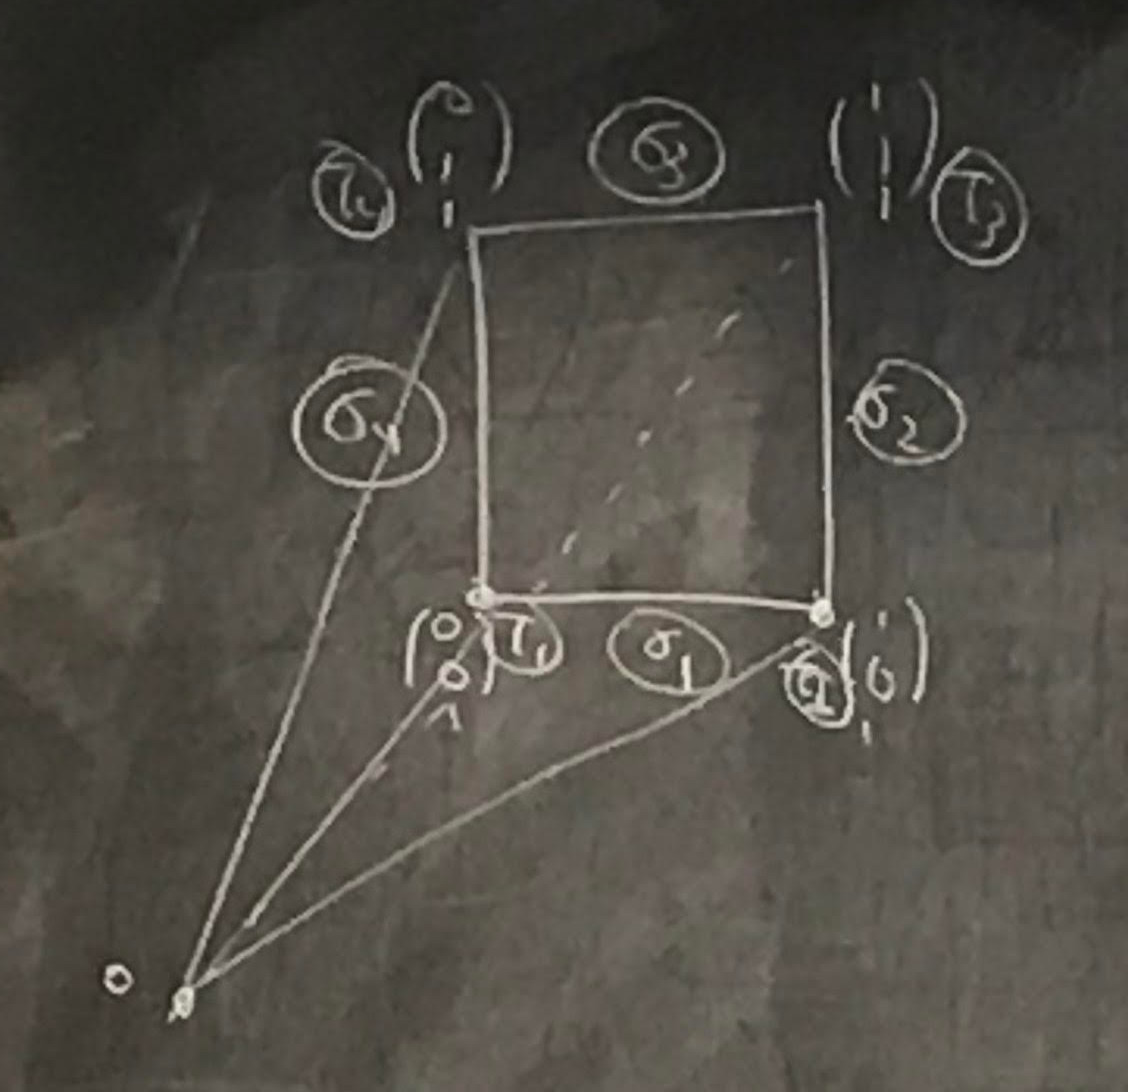
\includegraphics[scale=0.14]{pic/3}
\end{figure}

\begin{center}
	\begin{tabular}{ |c|c|c|c|c|c|} 
		\hline
		$\tau^*$ & $\tau$ & $dim\tau$ & $p_\tau \in \C^4$ & $dim V(\tau), dim O_\tau$ & ideal $V(\tau)$ \\
		\hline
		$0$ & $\sigma$ & $3$ & $(0,0,0,0)$ & $0$ & $(x_1,x_2,x_3,x_4)$ \\ 
		$x_1$ & $\sigma_1$ & $2$ & $(1,0,0,0)$ & $1 (\C^*)$ & $(x_2,x_3,x_4)$ \\
		$x_2$ & $\sigma_2$ & $2$ & $(0,1,0,0)$ & $1 $ & $(x_1,x_3,x_4)$ \\
		$x_3$ & $\sigma_3$ & $2$ & $(0,0,1,0)$ & $1 $ & $(x_1,x_2,x_4)$ \\
		$x_4$ & $\sigma_4$ & $2$ & $(0,0,0,1)$ & $1 $ & $(x_1,x_2,x_3)$ \\
		$x_1x_4$ & $\tau_1$ & $1$ & $(1,0,0,1)$ & $ 2 ((\C^*)^2) $ & $(x_2,x_3)$ \\
		$x_1x_2$ & $\tau_2$ & $1$ & $(1,1,0,0)$ & $2 $ & $(x_3,x_4)$ \\
		$x_2x_3$ & $\tau_3$ & $1$ & $(0,1,1,0)$ & $2 $ & $(x_1,x_4)$ \\
		$x_3x_4$ & $\tau_4$ & $1$ & $(0,0,1,1)$ & $2 $ & $(x_1,x_2)$ \\
		$\sigma^\vee$ & $0$ & $0$ & $(1,1,1,1)$ & $3 ((\C^*)^3) $ & $0$ \\
		\hline
	\end{tabular}
\end{center}


$$\sigma^\vee=\text{vcone}\bordermatrix{& x_1 & x_2 &\ x_3 & x_4 \cr
	& 0 &  1  & 0 & -1 \cr
	& -1  &  0 & 1 & 0 \cr
	& 0 & -1 & -1 & 0 }$$

$X_\sigma=V(x_1x_3-x_2x_4)$
$T=(\C^*)^3$
\\

$\tau\leq \sigma$:

$O_\tau:=T\cdot p_\tau$

$V(\tau):= \bar{O_\tau}\subseteq X_\sigma$ 

$X_\sigma\backslash X_\tau$
\\

$ p_{\sigma_1} $ ?

For any face $ \tau $, $p_\tau:$
\begin{align*}
	p_\tau : \sigma^\vee \cap M &\to \C\\
	m &\mapsto \begin{cases}
	1 & m\in \tau^\perp \\
	0 & m\not\in \tau^\perp
	\end{cases}
\end{align*}
$p_{\sigma_1}: \begin{cases}
x_1\mapsto 1 \\ x_2,x_3,x_4 \mapsto 0
\end{cases}$

$\sigma_1^\perp = span \left( \begin{array}{c}  0 \\ -1 \\ 0 \end{array}  \right)$

$ p_{\tau_1}:$

$\tau_1^\vee=span(x_1,x_4)$

$p_{\tau_1}=(1,0,0,1) $
\\

Theorem Discovery Time:

$\tau\leq \sigma$ ($\sigma$ pointed cone, $dim
\sigma= rkN=n$)
\begin{enumerate}[1)]
\item $O_\tau \simeq (\C^*)^{n-dim\tau}$\\
so  $ dim O_\tau= n-=dim\tau $\\
so $dimV(\tau) =n-dim\tau$
\item $ V(0)=x_\sigma $\\
$ V(\sigma) =  $ origin $=$ single point $P_\sigma$
\item Orbits are disjoint: $ \tau_1, \tau_2 \leq \sigma, \tau_1\neq \tau_2 \Rightarrow O_{\tau_1} \cap O_{\tau_2} = \emptyset $
\item $ X_\sigma = \sqcup _{\gamma\leq \sigma} O_\gamma $
\end{enumerate}
Write $ X_\tau, V(\tau) $ as unions of orbits
\\

$X_\tau=\sqcup_{\gamma\leq \tau} O_\gamma$ - toric variety

$ V(\tau) = \sqcup_{\tau\leq \gamma} O_\gamma $ - toric variety (needs a bit of proof)

$ X_\sigma\backslash X_\tau =\sqcup_{not(\gamma\leq \tau)}O_\gamma $ - not toric
\\

$ X_\sigma \backslash (\C^*)^n = \cup_{\tau codim 1, \text{in }\sigma} V(\tau) $

(note: if $ \tau \leq \sigma$ then $ X_\tau \hookrightarrow X_\sigma $)
\\

\begin{Theorem}
	Let $ \sigma =$ (pointed) cone in $N$, $ rk(N)=n=dim\sigma $
	\begin{enumerate}[a)]
		\item There exists a bijection
		\begin{align*}
			\{\text{faces }\tau \in \sigma\} &\xleftrightarrow{1-1} \{T\text{-orbits of }X_\sigma\}\\
			\tau &\mapsto T\cdot p_\tau = O_\tau
		\end{align*}
		\item $dimO_\tau = n-dim\tau$ (for $\tau \leq \sigma$)
		
		$O_\tau \simeq (\C^*)^{n-dim\tau}$
		
		$dimV(\tau)=n-dim\tau$
		\item If $ \tau \leq \sigma$, $X_\tau=\sqcup_{\gamma\leq \tau} O_\gamma $
		\item $ V(\tau)=\sqcup_{\tau\leq\gamma} O_\gamma $
		\item $ V(\tau) $ is an affine toric variety
	\end{enumerate}
\end{Theorem}

\subsection{Affine Toric Morphisms}

Suppose $\phi:N'\to N$ is a group homomorphism ($N, N'$ are lattices) and suppose $\sigma'$ is a cone in $N'$, $\sigma$ is a cone in $N$ such that $\phi_\R: N_\R'\to N_\R$ satisfies $\phi_\R(\sigma')\subseteq \sigma$
\\

(notational issue: for us, $\sigma$ cone in $N$ $\leadsto X_\sigma = Spec\C[\sigma^\vee \cap M]$

$X_\sigma$ depends on $\sigma$, and on $N$ (also $M$):

$X_\sigma = X_{\sigma,N}$

for us: $N$ is ``understood"
)
\\

Want: $X_{\sigma'}\to X_\sigma$ (or is it $X_\sigma \to X_{\sigma'}$?)
\\

$ \phi: N'\to N $

so  $ \phi^*: M\to M' $.

$ \phi(\sigma')\subseteq \sigma $

so $\phi^*(\sigma\vee)\subseteq \sigma'^\vee$.

So we get a map:

$\sigma^\vee\cap M\to \sigma'^\vee \cap M'$

Therefore, $\C[\sigma^\vee \cap M] (=A_\sigma)\to \C[\sigma'^\vee \cap M'](=A_{\sigma'})$.

$\phi:X_{\sigma'}\to X_\sigma$
\\

A morphism $X_{\sigma'}\to X_\sigma$ is called an (affine) toric morphism if it is of this form.
\\

\begin{Eg}
	\begin{figure}[htbp]\centering
		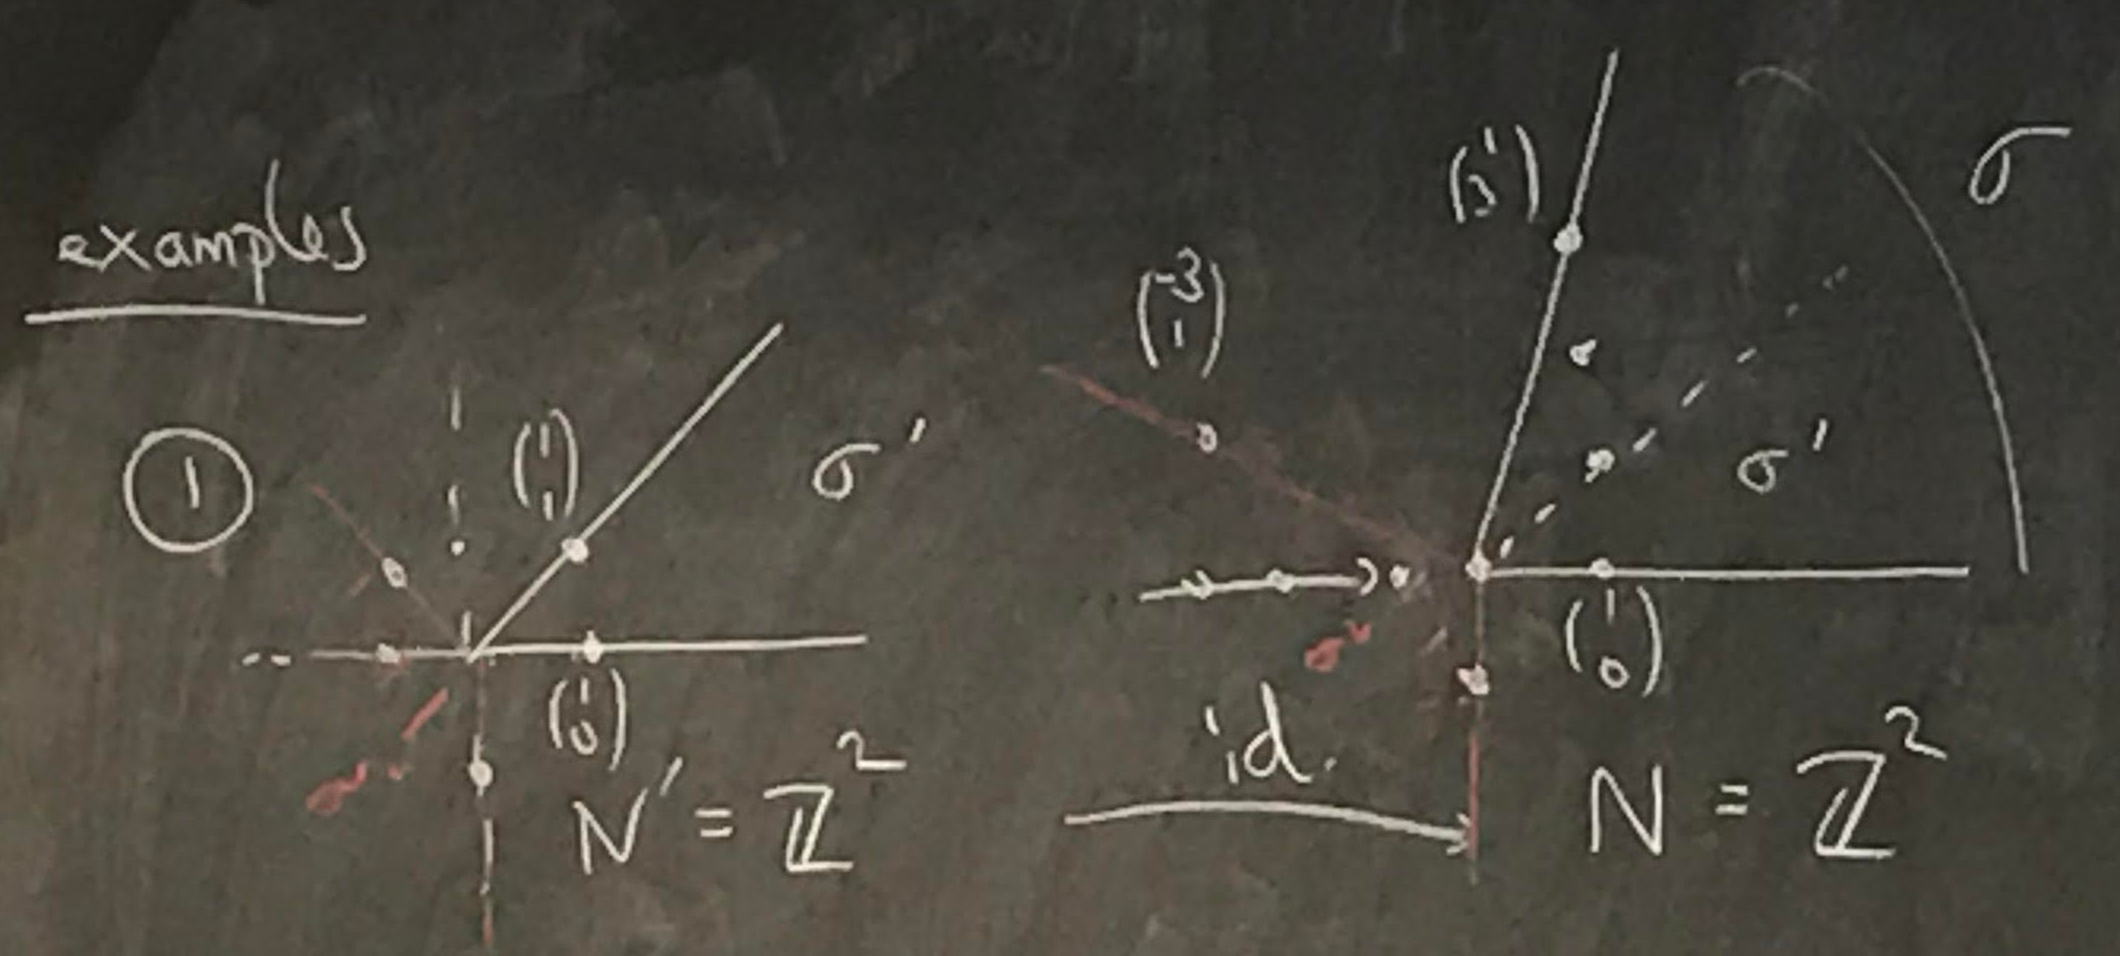
\includegraphics[scale=0.15]{pic/1}
	\end{figure}
\begin{enumerate}[1)]
	\item $\sigma' \subseteq \sigma\leadsto X_{\sigma'}\to X_\sigma$
	
	$X_{\sigma'}=Spec\C[t\iv, s\iv t]=\C[y_1,y_2]\simeq \C^2$
	
	$X_\sigma = Spec\C[s\iv, s^{-3}t, t\iv] \simeq Spec\C[x_1,x_2,x_3]/(x_1^3-x_2x_3)$
	\\
	
	$X_{\sigma'}\to X_\sigma$
	
	$\C^2\to X_\sigma\subseteq \C^3$
	
	$(y_1,y_2)\mapsto (y_1y_2,y_1^2y_2^3,y_1)$
	
	$V(y_1)\subseteq \C^2 \mapsto (0,0,0)$
	\item  $N'=\Z^2 \subseteq N=\{(\frac{a}{2},\frac{b}{2}): a,b\in \Z, a+b\equiv 0 (mod 2) \}$
	
	$\sigma'=\sigma = vcone \begin{pmatrix} -1 & 0 \\ 0 & -1 \end{pmatrix}$
	
	$M'=\Z^2 \supseteq M= \{(a,b): a,b,\in Z, a+b\equiv 0 (mod2)\}$
	
	\begin{figure}[htbp]\centering
		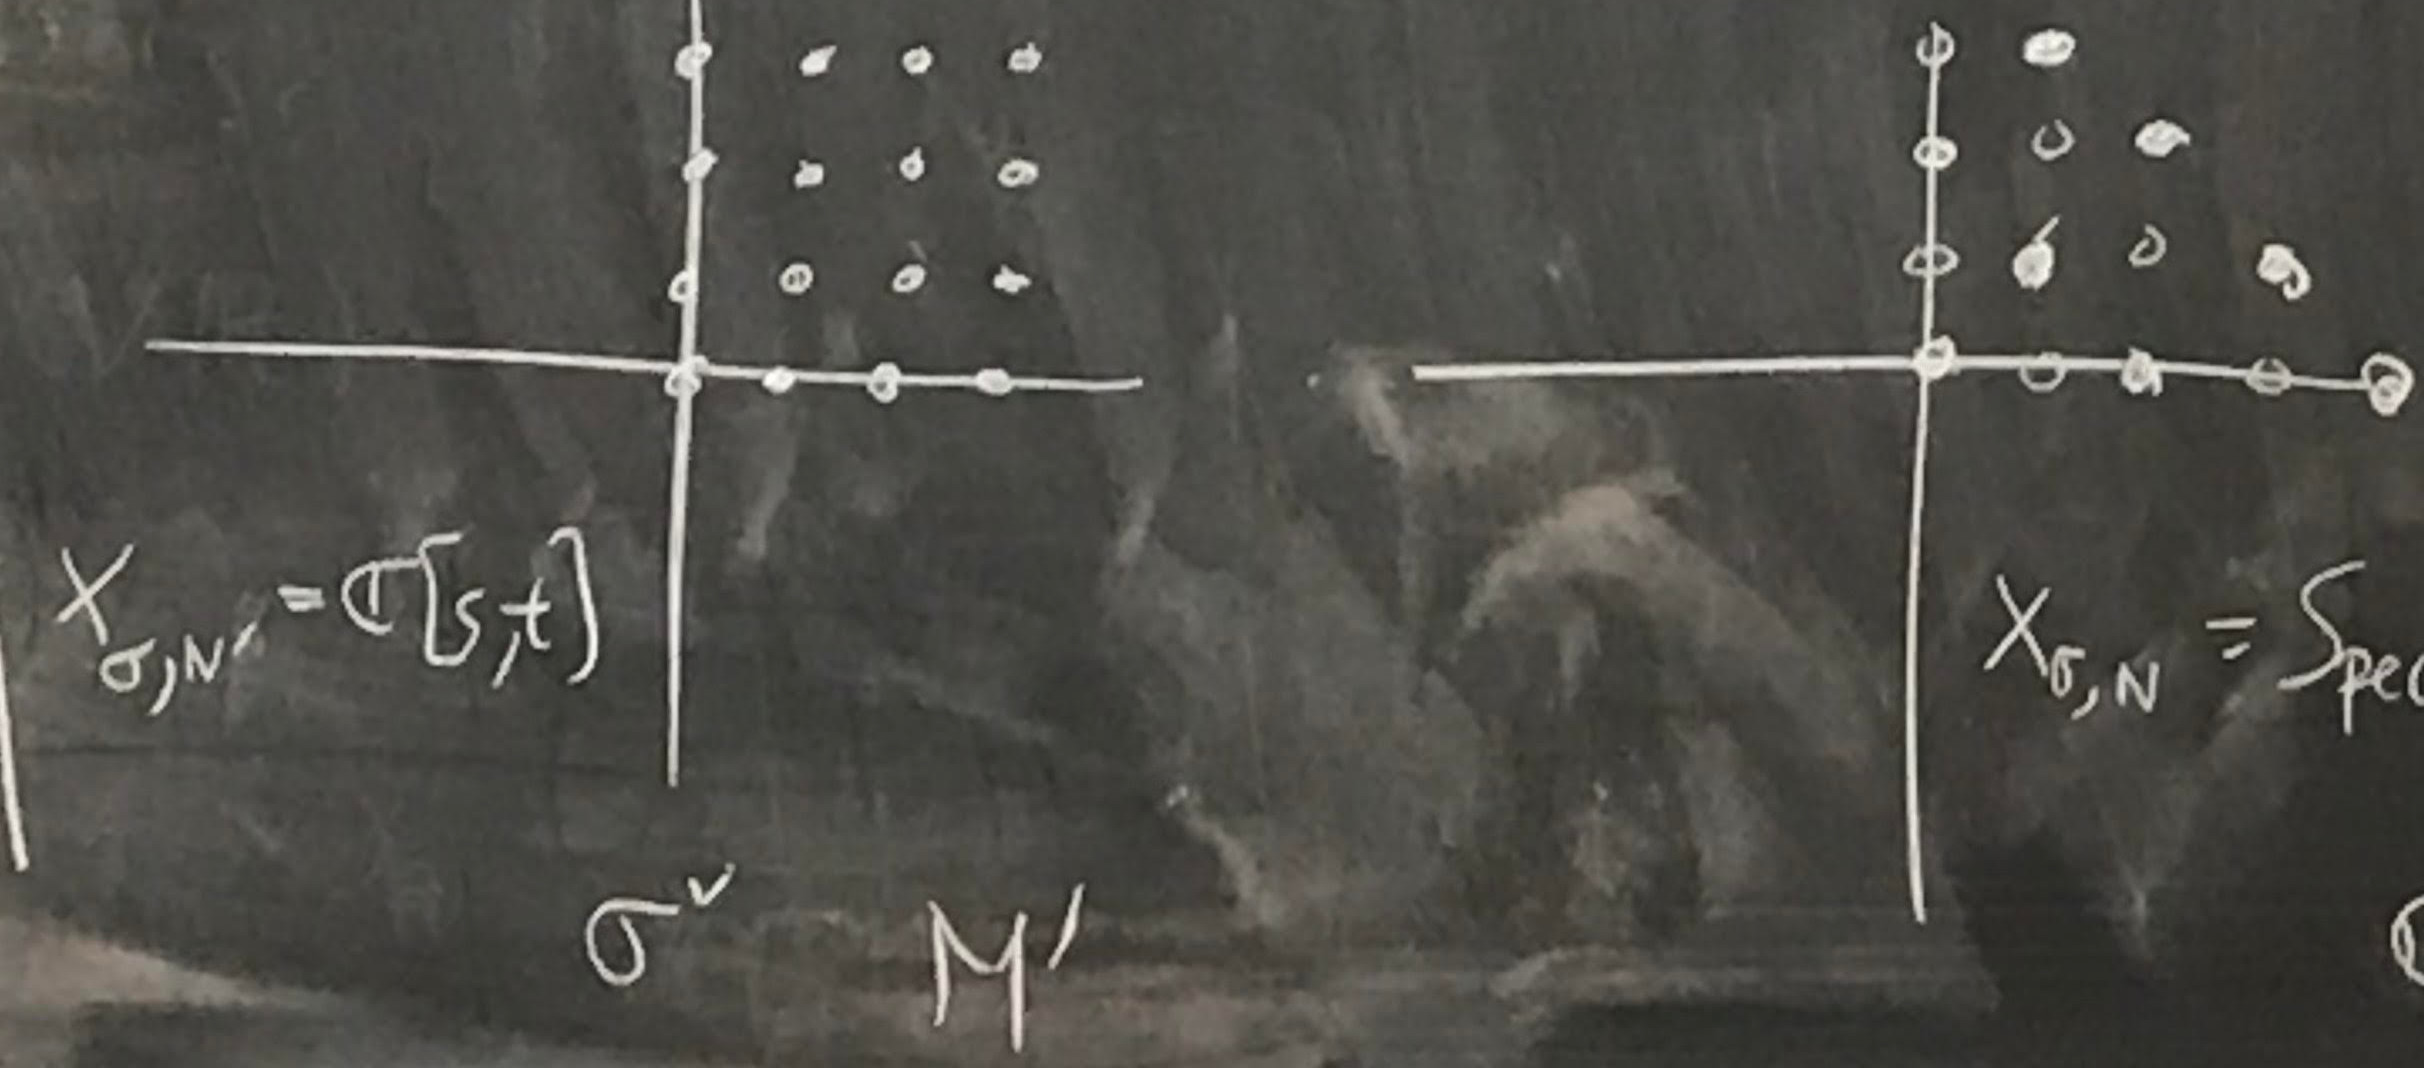
\includegraphics[scale=0.1]{pic/2}
	\end{figure}
	
	$X_{\sigma,N'}=\C[s,t]$
	
	$X_{\sigma,N}=Spec\C[s^2,st,t^2]=Spec()\C[x_1,x_2,x_3]/(x_1x_3-x_2^2))(=X)$
	
	$\C^2\to X$
	\\
	
	$\C^2\xrightarrow{2-1} X$
	
	$(x,y)\mapsto (x^2,xy,y^2)$
\end{enumerate}
\end{Eg}

\newpage
\section{Lecture February 19}

\subsection{General Toric Varieties}
Glueing Construction:
\begin{Def}["glueing data"]
	Suppose we are given the following:
	\begin{enumerate}[a)]
		\item A finite number of affine varieties (irreducible) $ \{V_\alpha: \alpha\in \Lambda\} $
		\item All $\alpha, \beta \in \Lambda$, a (nonempty, dense) Zariski open subset $V_{\beta\alpha}\subseteq V_\alpha$.
		\item All $\alpha, \beta \in \Lambda$, an isomorphism $ g_{\beta\alpha}: V_{\beta\alpha}(\subseteq V_\alpha)\xrightarrow{\sim}V_{\alpha\beta}(\subseteq V_\beta) $
		
		$x\in V_{\beta\alpha}\subseteq V_\alpha$, $g_{\beta\alpha}(x)\in V_{\alpha\beta}\subseteq V_\beta$
		
		such that
		\begin{enumerate}[1)]
			\item $V_{\alpha\alpha}=V_\alpha$, $g_{\alpha\alpha}=id_{V_\alpha}$
			\item All $\alpha, \beta \in \Lambda, g_{\alpha\beta}=g_{\beta\alpha}\iv$
			\item All $\alpha, \beta, \gamma \in \Lambda$,
			
			$g_{\beta\alpha}(V_{\beta\alpha}\cap V_{\gamma\alpha})(\subseteq V_\alpha)=V_{\alpha\beta}\cap V_{\gamma\beta}(\subseteq V_\beta)$
			
			and on $V_{\beta\alpha}\cap V_{\gamma\alpha}: g_{\gamma\alpha}=g_{\gamma\beta}g_{\beta\alpha}$
		\end{enumerate}
	\end{enumerate}
\end{Def}
Given this glueing data,
construct a set $V:=\sqcup_{\alpha\in\Lambda} V_\alpha$ (disjoint union).

Define $a\sim b$ if there exists $\alpha, \beta$ such that $a\in V_{\beta\alpha}, b\in V_{\alpha\beta}$ and $g_{\beta\alpha}(a)=b$.

Let $X:=V/\sim$.

This inherits the quotient topology.

\begin{Eg}
	$U_\alpha=\{[a]: a\in V_\alpha\}\subseteq X$ is an open set, 
	and $h_\alpha: V_\alpha\to U_\alpha, a\mapsto[a]$ is a homeomorphism.
	
	Thus, $X$ is "locally an affine variety."
\end{Eg}
Such an $X$ is called an abstract variety.
\\
\begin{Eg}[Key example: $\mathbb{P}^n_{x_1\cdots x_n}$]
	Let $U_i:=\mathbb{P}^n\backslash V(x_i)\simeq \C^n=Spec\C[\frac{x_0}{x_i},\frac{x_1}{x_i},...,\hat{\frac{x_i}{x_i}},...,\frac{x_n}{x_i}]=Spec\C[t_{i2},t_{i2},...,t_{in}]$
	
	$\Lambda=\{0,...,n\}$
	
	$V_i=\C^n=Spec\C[\frac{x_0}{x_i},...,\frac{x_n}{x_i}]$
	
	$V_{ji}=Spec\C[\frac{x_0}{x_i},...,\frac{x_n}{x_i}]_{\frac{x_j}{x_i}}$
	\\
	
	$g_{ji}:V_{ji}\to V_{ij}$ corresponds to
	
	$\C[\frac{x_0}{x_j},...,\frac{c_n}{x_j}]_{\frac{x_i}{x_j}}\xleftrightarrow{id}\C[\frac{x_0}{x_i},...,\frac{x_n}{x_i}]_{\frac{x_j}{x_i}}$
	
	Glue: $\{U_i,U_{ji},g_{ji}\}$ together: get $\mathbb{P}^n$.
\end{Eg}

\subsection{Regular functions}
What are regular functions/morphisms(=regular map)?

Let $X=\cup_{\alpha \in \Lambda} U_\alpha$ be an abstract affine variety. Let $U\subseteq X$ be an open subset. 

Then a function $\phi:U\to \C$ is called regular (on $U$) if the restriction [$W_\alpha:=h_\alpha\iv(U\cap U_\alpha)\subseteq V_\alpha$ is open] $\phi h_\alpha: W_\alpha \to \C$ is regular.
\\
\begin{Def}Assume that $X=\cup_{\alpha \in \Lambda}U_\alpha$ is an abstract variety.
	Define $ \mathcal{O}_X(U)=\{\phi:U\to C: \phi \text{ is regular } \}$.
\end{Def}
\begin{Proposition}
	These $\mathcal{O}_X(U)$'s piece together to form a sheaf of rings $\mathcal{O}_X$.
\end{Proposition} 
Therefore $(X,\mathcal{O}_X)$ is a scheme.
\\

Let $X=\cup_{\alpha\in \Lambda}U_\alpha$, $Y=\cup_{\beta \in \Lambda'}U'_\beta$.

A morphism (or regular map) $f:X\to Y$ is a continuous map $X\to Y$ such that for all $\alpha \in \Lambda$, $\beta \in \Lambda'$:

$f|_{U_\alpha\cap f\iv(U_\beta')}:U_\alpha\cap f\iv(U_\beta')\xrightarrow{f}U_\beta'$ is regular.
\\

Let's glue a bunch of affine toric varieties together. 

Let $\Sigma$ be our index set.
\\

A) Need for $\alpha \in \Sigma$, need an affine toric variety $V_\alpha$ (let $\Sigma$ be a finite set of (pointed) cones in $N=\Z^n$, let $V_\alpha := X_\alpha, \alpha \in \Sigma$)
\\

(Lightbulb!) If $\tau=\text{face of } \alpha$, $X_\tau\hookrightarrow X_\alpha$ is Zariski open.

If also $\tau=\text{face of }\beta $, $X_\tau \hookrightarrow X_\beta$ (Zariski open as well).
\\

B) Need for $\alpha, \beta \in \Sigma$ an open subset $V_{\beta\alpha}\subseteq V_\alpha$

ASSUME if $\alpha,\beta \in \Sigma$ then $\alpha \cap \beta$ is a face of $\alpha$, and of $\beta$.

Then, $V_{\beta\alpha}:= V_\tau \hookrightarrow V_\alpha$ if $\tau = \alpha\cap \beta \leq \alpha$

$g_{\beta\alpha}:V_{\beta\alpha}(=V_\tau)\xrightarrow{id}V_{\alpha\beta}(=V_\tau)$.
\\

Triple intersections:
$V_{\beta\alpha}\cap V_{\gamma\alpha}(=V_{\alpha\cap\beta\cap \gamma})``=" V_\alpha\cap V_\beta\cap V_\gamma$.
\\

\begin{Def}[Version 0.1]
	A fan $\Sigma$ in $N_\R$ is a finite collection of (pointed) cones in $N$ satisfying:
	\begin{enumerate}[a)]
		\item if $\tau\leq \sigma\in \Sigma$, then $\tau\in \Sigma$
		\item For all $\alpha, \beta \in \Sigma$, then $\alpha\cap \beta\in\Sigma$, and is a fan of $\alpha$ and of $\beta$.
	\end{enumerate}
\end{Def}

\begin{Eg}[not a fan]$\Sigma=\{\sigma, \sigma',\tau,\text{ other faces of }\sigma, \sigma'\}$
\begin{figure}[h!]\centering
	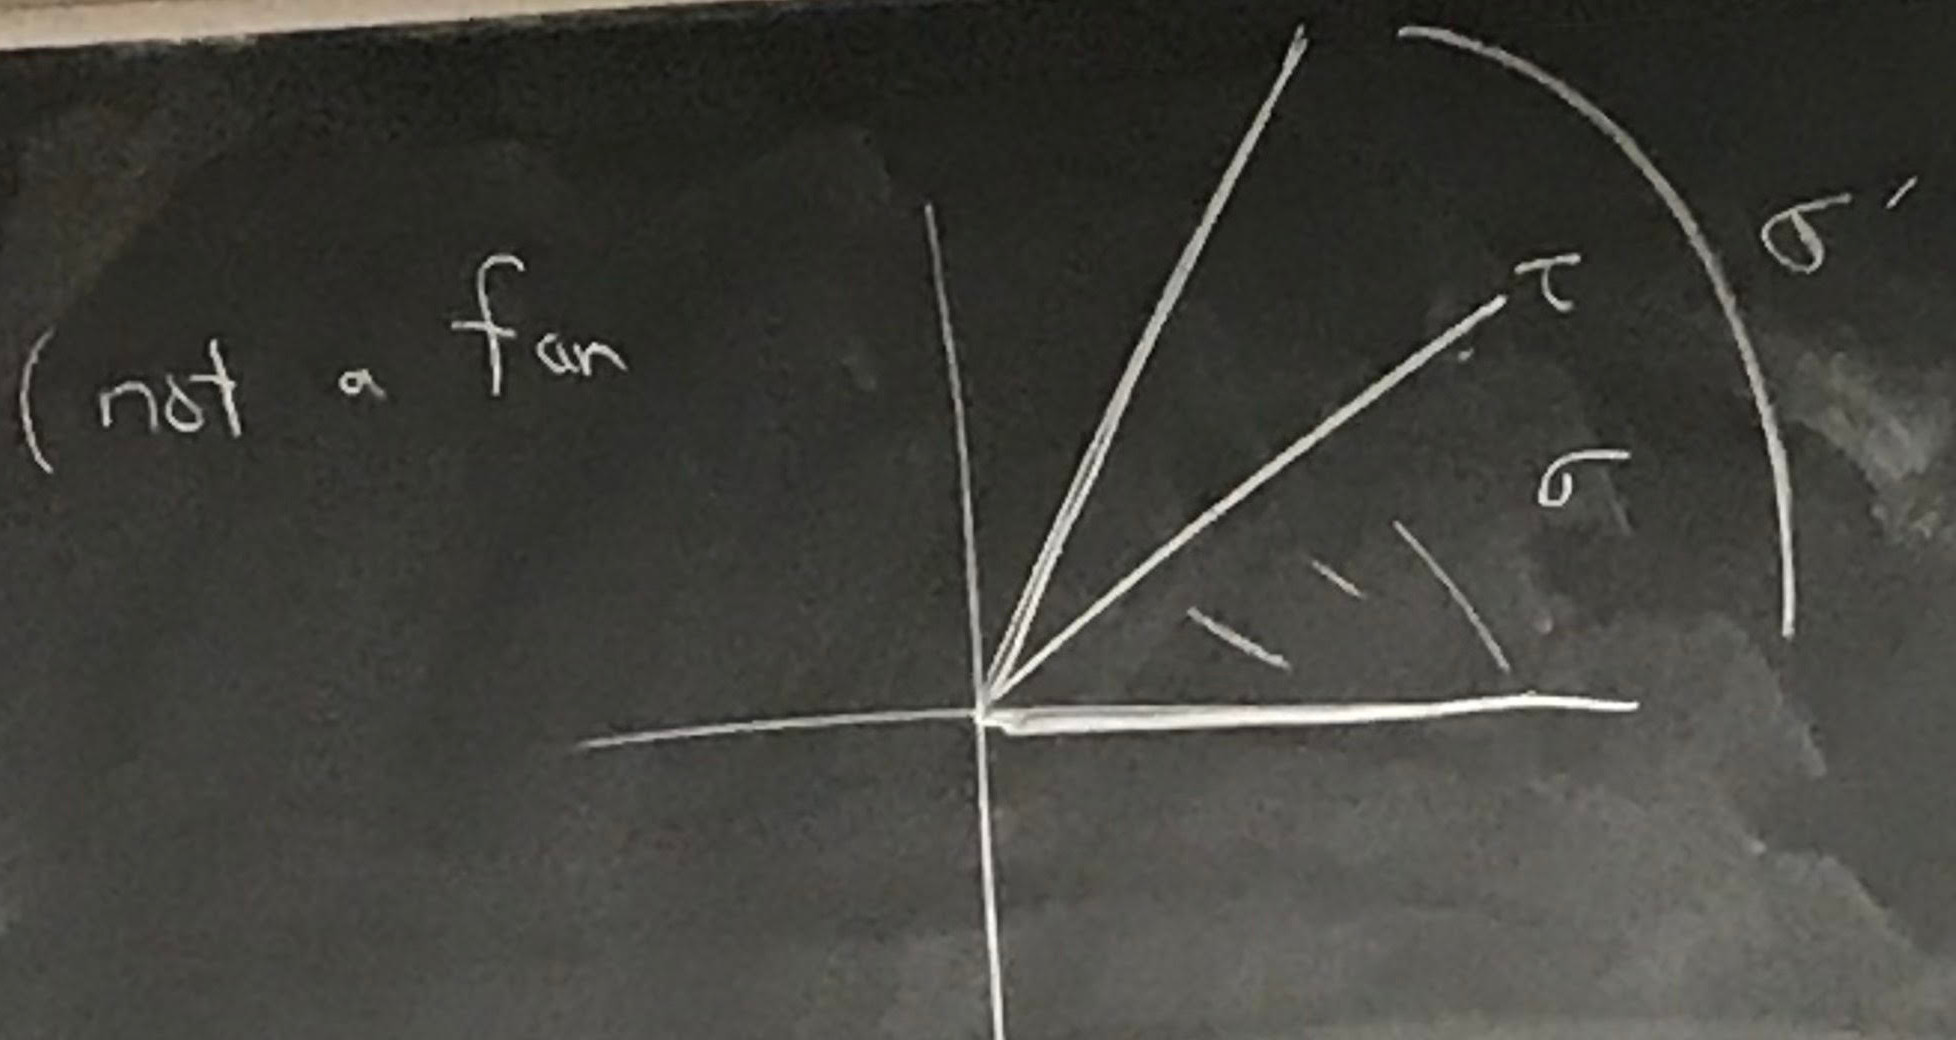
\includegraphics[scale=0.1]{pic/4}
\end{figure}
\end{Eg}
Some notions
\begin{enumerate}[a)]
	\item The support of $\Sigma$ is $|\Sigma|:=\cup_{\sigma\in\Sigma}\sigma \subseteq N_\R$.
	\item $\Sigma(r):=\{\sigma\in\Sigma, \text{dim}\sigma=r\}$
	\item $\Sigma_{max}:=\{\sigma \in \Sigma: \text{dim}\sigma\text{ maximal }= n\}$
	\item $ \Sigma $ is called complete if $|\Sigma|=N_\R$.
	\item $\Sigma$ is called simplicial if every $\sigma \in \Sigma$.
	\item $\Sigma$ is called smooth if every $\sigma\in \Sigma$ is smooth.
\end{enumerate}

\newpage
\section{Back to Fans}

\begin{Def}
	A {\bf fan} $\Sigma$ in $N_{\mathbb{R}}$ is a finite collection of cones $\sigma \in N_{\mathbb{R}}$ satisfying:
	\begin{enumerate}
		\item If $\sigma \in \Sigma$ then $\sigma$ is a rational polyhedral cone (in $N_{\mathbb{R}}$).
		\item If $\tau \leq \sigma \in \Sigma$ is a face then $\tau \in \Sigma$.
		\item For all $\sigma_1, \sigma_2 \in \Sigma$ then $\tau := \sigma_1 \cap \sigma_2$ must be a face of both $\sigma_1, \sigma_2$ (and hence $\tau \in \Sigma$).
	\end{enumerate}
\end{Def}

\begin{Eg}~\\
	
	\begin{figure}[h]
		\begin{center}
			\begin{tikzpicture}
			\draw[step=1cm,gray,very thin] (-3.9,-3.9) grid (3.9,3.9);
			\draw[thick,->] (-3.9,0) -- (3.9,0);
			\draw[thick,->] (0,-3.9) -- (0,3.9);
			\draw[very thick, red, ->] (0,0) -- (3.9,3.9) node[anchor=south east] {$\sigma_1$};
			\draw[very thick, red, ->] (0,0) -- (-3.9,2) node[anchor = south west]{$\sigma_3$};
			\draw[very thick, red, ->] (0,0) -- (2.5,-3.9) node[anchor=north east]{$\sigma_2$};
			\node[red] at (-0.5,2.5) {$\alpha_3$};
			\node[red] at (-1.5,-1.5){$\alpha_2$};
			\node[red] at (2.5,0.5){$\alpha_1$};
			\node at (-0.25,-0.25){0};
			\end{tikzpicture}
		\end{center}
	\end{figure}
	
	Let $\Sigma = \{ \sigma_1, \sigma_2, \sigma_3, 0\}$ and let $\tilde{\Sigma} = \{\alpha_1,\alpha_2,\alpha_3,\sigma_1,\sigma_2,\sigma_3, 0\}$.
\end{Eg}

\begin{Theorem}
	Let $\Sigma$ be a fan in $N_{\mathbb{R}}$.  Let $V_{\alpha} := X_{\alpha}$ for $\alpha \in \Sigma$, let $V_{\beta \alpha} := V_{\alpha \cap \beta} \subseteq V_{\alpha}$ for all $\alpha, \beta \in \Sigma$ and let 
	\begin{center}
		\begin{tikzcd}
			g_{\beta \alpha}: &V_{\beta \alpha}  \arrow[d, equal] \arrow[r] & V_{\alpha\beta} \arrow[d, equal] \\
			&\tau \arrow{r}{\text{id}} &\tau.
		\end{tikzcd}
	\end{center}
	Then these data satisfy the glueing axioms.  Let $X_{\Sigma}$ denote the resulting abstract variety.  Then $X_{\Sigma}$ is  reduced, irreducible, separated and of finite type over $\mathbb{C}$.
\end{Theorem}

We have 
\[X_{\Sigma} = \bigcup_{\alpha \in \Sigma} U_{\alpha}\]

and $U_{\alpha} \simeq X_{\alpha}$ is a dense open subset of $X_{\Sigma}$ (in fact, $\{U_{\alpha}: \alpha \in \Sigma_{\text{max}}\}$ is an open cover of $X_{\alpha}$).
\newpage
\begin{exercise}
	Identify the varieties $X_{\Sigma}$ in the following examples:
	\begin{enumerate}[(a)]
		\item ~\\
		
		\begin{figure}[h]
			\begin{center}
				\begin{tikzpicture}
				\draw[step=1cm,gray,very thin] (-3.9,-3.9) grid (3.9,3.9);
				\draw[thick,->] (-3.9,0) -- (3.9,0);
				\draw[thick,->] (0,-3.9) -- (0,3.9);
				\draw[very thick, red] (0,0) -- (0,3.9) node[anchor=north east] {$e_2$};
				\draw[very thick, red, ->] (0,0) -- (-3.9,-3.9) node[anchor = south west]{$-e_1-e_2$};
				\draw[very thick, red, ->] (0,0) -- (3.9,0) node[anchor=north east]{$e_1$};
				\node[red] at (1.5,1.5) {$\sigma_1$};
				\node[red] at (-2.5,1.5){$\sigma_2$};
				\node[red] at (0.5,-2.5){$\sigma_3$};
				\node at (-0.25,-0.25){0};
				\end{tikzpicture}
			\end{center}
		\end{figure}
		(Show that $X_{\Sigma} = \mathbb{P}^2$.)
		\item ~\\
		
		\begin{figure}[h]
			\begin{center}
				\begin{tikzpicture}
				\draw[step=1cm,gray,very thin] (-3.9,-3.9) grid (3.9,3.9);
				\draw[thick,->] (-3.9,0) -- (3.9,0);
				\draw[thick,->] (0,-3.9) -- (0,3.9);
				\draw[very thick, red] (0,0) -- (0,3.9) node[anchor=north east] {$e_2$};
				\draw[very thick, red] (0,0) -- (3.9,0) node[anchor=south east] {$e_1$};
				\draw[very thick, red, ->] (0,0) -- (-3.9,0) node[anchor = south west]{$-e_1$};
				\draw[very thick, red, ->] (0,0) -- (0,-3.9) node[anchor=south east]{$-e_2$};
				\node[red] at (1.5,1.5) {$\sigma_1$};
				\node[red] at (-1.5,1.5){$\sigma_2$};
				\node[red] at (-1.5,-1.5){$\sigma_3$};
				\node[red] at (1.5,-1.5){$\sigma_4$};
				\node at (-0.25,-0.25){0};
				\end{tikzpicture}
			\end{center}
		\end{figure}
		(Show that $X_{\Sigma}= \mathbb{P}^1 \times \mathbb{P}^1$.)
	\end{enumerate}
\end{exercise}
\newpage
\begin{Proposition}
	Let $\sigma$ be a cone in $N$.\\
	Let $u \in \sigma^{\vee} \cap M$.\\
	Let $\tau := \sigma \cap u^{\perp}$ be a face of $\sigma$.\\
	Then $S_{\tau} = S_{\sigma}+\mathbb{Z}_{\geq 0}(-u)$.
\end{Proposition}

\begin{figure}[h!]
	\begin{center}
		\begin{tikzpicture}
		\draw[step=1cm,gray,very thin] (-3.4,-3.4) grid (3.4,3.4);
		\draw[thick,->] (-3.4,0) -- (3.4,0);
		\draw[thick,->] (0,-3.4) -- (0,3.4);
		\draw[very thick, red] (0,0) -- (2.5,3) node[anchor=north west] {$\tau$};
		\draw[very thick, red] (0,0) -- (3,1.5);
		\draw[very thick, blue] (0,0) -- (-3,2.5) node[anchor = south west]{$u$};
		\draw[very thick, blue, dashed] (0,0) -- (3,-2.5);
		\draw[very thick, blue] (0,0) -- (1.5,-3);
		\node[red] at (1.75,1.5) {$\sigma_1$};
		%\node[red] at (-1.5,1.5){$\sigma_2$};
		\node[blue] at (-1.5,-1.5){$\sigma^{\vee}$};
		%\node[red] at (1.5,-1.5){$\sigma_4$};
		\node at (-0.25,-0.25){0};
		\end{tikzpicture}
	\end{center}
\end{figure}

\begin{Proposition}[Separation lemma]  Suppose $\sigma, \sigma'$ are convex polyhedral cones such that $\tau = \sigma\cap \sigma'$ is a face of both.  Then for all $u \in \text{rel int}(\sigma^{\vee} \cap(-\sigma')^{\vee})$, $\tau = \sigma \cap u^{\perp} = \sigma'\cap u^{\perp}$.
\end{Proposition}

\begin{figure}[h!]
	\begin{center}
		\begin{tikzpicture}
		\draw[step=1cm,gray,very thin] (-3.4,-3.4) grid (3.4,3.4);
		\draw[thick,->] (-3.4,0) -- (3.4,0);
		\draw[thick,->] (0,-3.4) -- (0,3.4);
		\draw[very thick, blue] (0,0) -- (2,3) node[anchor=north west] {$\tau$};
		\draw[very thick, blue] (0,0) -- (-2,-3) node[anchor=south east] {$-\tau$};
		\draw[very thick, red] (0,0) -- (3.5,2.5);
		\draw[very thick, green, dashed] (0,0) -- (-3,2) node[anchor= south west] {$\sigma^{\vee} \cap (-\sigma')^{\vee}$};
		\draw[very thick, red] (0,0) -- (-1,-4);
		\node[red] at (1.75,1.5) {$\sigma_1$};
		%\node[red] at (-1.5,1.5){$\sigma_2$};
		\node[red] at (-1.3,-2.8){$-\sigma'$};
		%\node[red] at (1.5,-1.5){$\sigma_4$};
		\node at (-0.25,-0.25){0};
		\end{tikzpicture}
	\end{center}
\end{figure}

\begin{Proposition}
	If $\sigma, \sigma'$ are cones in $N$ such that $\tau = \sigma \cap \sigma'$ is a face of each, then $S_{\tau} = S_{\sigma}+ S_{\sigma'}$.
	\begin{Remark}
		Proofs can be found in Fulton.
	\end{Remark}
\end{Proposition}

\newpage
\section{Polytopes and polyhedra}

\begin{Def}
	A {\bf polytope} $P$ in $V= \mathbb{R}^n$ is the convex hull 
	\begin{align*}
		P&= \text{conv}(v_1, \ldots, v_r) \quad \text{ for some } v_i \in V\\
		&= \{t_1v_1 + \ldots + t_r v_r : t_i \geq 0, \sum t_i = 1\}
	\end{align*}
\end{Def}

\begin{Def}
	A {\bf Polyhedron} $P$ in $V=\mathbb{R}^n$ is the intersection of finitely many affine half spaces, i.e. there exist $A\in\mathbb{R}^{m\times n}, b \in \mathbb{R}^m$ such that
	\[ P = \{x \in \mathbb{R}^n : Ax=b\}\]
	(one row corresponds to one half space).
\end{Def}

\begin{Eg}
	\begin{enumerate}
		\item ~\\
		\begin{figure}[h!]
			\begin{center}
				\begin{tikzpicture}
				\draw[thick] (0,0) -- (5,0) -- (2,1) -- (0,1) -- (0,0);
				\node[below left] at (0,0){(0,0)};
				\node[below right] at (5,0){(5,0)};
				\node[above right] at (2,1){(2,1)};
				\node[above left] at (0,1){(0,1)};
				\end{tikzpicture}
			\end{center}
		\end{figure}
		
		This is both a polytope and a polyhedron.
		\item ~\\
		
		\begin{figure}[h!]
			\begin{center}
				\begin{tikzpicture}
				\filldraw[fill=red!20!white, draw=red!20!white] (0,3.9) -- (0,1) -- (1,0) -- (3.9,0) -- (3.9,3.9);
				\draw[thick,->] (-0.9,0) -- (3.9,0);
				\draw[thick,->] (0,-0.9) -- (0,3.9);
				\draw[ultra thick, red] (1,0) -- (3.9,0);
				\draw[ultra thick, red] (0,1) -- (0,3.9);
				\draw[ultra thick, red] (0,1) -- (1,0);
				\node[red] at (2,2){P};
				\end{tikzpicture}
			\end{center}
		\end{figure}
		This is a polyhedron but not a polytope:
		\[P = \left\{(x,y)\in \mathbb{R}^2 : \begin{pmatrix}
		-1 & 0\\
		0 &-1 \\
		-1 &-1
		\end{pmatrix}
		\begin{pmatrix} x \\ y\end{pmatrix} \leq 
		\begin{pmatrix} 0 \\ 0 \\ -1 \end{pmatrix} \right\}\]
	\end{enumerate}
\end{Eg}

\begin{Def}
	If $P = \text{conv}(v_1, \ldots, v_r)$ is a polytope, the {\bf cone over $P$} is 
	\[ C(P) := \text{vcone} \begin{bmatrix} 1 & 1 & \ldots & 1 \\ v_1 &v_2 & \ldots & v_r \end{bmatrix} \subseteq \mathbb{R}\oplus V = \mathbb{R}^{n+1} \]
\end{Def}

\noindent {\bf Simple Fact \# 1:} $x \in P \iff \begin{pmatrix} 1 \\ x \end{pmatrix} \in C(P)$.

\noindent {\bf Check:} 
\begin{align*}
	x\in P &\iff \exists t_1, \ldots, t_r \geq 0, \sum t_i = 1 \text{ such that } x = \sum t_i v_i\\
	&\iff \begin{pmatrix} 1 \\ x \end{pmatrix} = t_1 \begin{pmatrix} 1 \\ v_1 \end{pmatrix} + \ldots + t_r  \begin{pmatrix} 1 \\ v_r \end{pmatrix}  \text{ for some } t_i \geq 0.
\end{align*}

\begin{Corollary}
	If $P$ is a polytope then $P$ is a polyhedron.
\end{Corollary}

\begin{proof}
	$C(P)$ is a polyhedral cone by construction, so there exists a matrix $B \in \mathbb{R}^{m \times (n+1)}$ such that
	\[ C(P) = \{ y\in \mathbb{R}^{n+1} : By \leq 0\} \]
	with $B = [-b \ \ A] $ for $b\in \mathbb{R}^m$, $A \in \mathbb{R}^{m\times n}$, then 
	\[C(P) = \{y \in \mathbb{R}^{n+1}: [-b \ \ A]y \leq 0\} \]
	now
	\begin{align*}
		P &= \left\{ x \in \mathbb{R}^{n} : \begin{pmatrix} 1 \\ x \end{pmatrix} \in C(P) \right\}\\
		&= \{x \in \mathbb{R}^n : -b +Ax \leq 0\} \\
		&= \{ x\in \mathbb{R}^n : Ax \leq b\}
	\end{align*}
\end{proof}

\begin{Remark}
	If $P$ is a polytope then $P$ is bounded.
\end{Remark}

\begin{Def}
	Let $P$ be a polyhedron as above.  The {\bf homogenisation} $C(P) \subseteq \mathbb{R} \oplus V = \mathbb{R}^{n+1}$ (coordinates $x_0, x_1, \ldots, x_n$) of $P$ is:
	\[ C(P) : = \{ y\in \mathbb{R}\oplus V : [-b \ \ A] y \leq 0, y_0 \geq 0\}\]
\end{Def}

\begin{Note}
	$C(P)$ is a polyhedral cone.
\end{Note}

\begin{Remark}
	If $P$ is a polytope and a polyhedron then
	\[C(P)_{\text{tope}} = C(P)_{\text{hedron}}\]
\end{Remark}


\noindent {\bf Simple Fact \# 2:} Let $P$ be a polyhedron, then
\[ x\in P \iff \begin{pmatrix} 1 \\ x \end{pmatrix} \in C(P)\]

\begin{proof}
	\begin{align*}
		x \in P &\iff Ax \leq b\\
		&\iff [-b \ \  A] \begin{pmatrix}1\\x \end{pmatrix} \leq 0 \\
		&\iff \begin{pmatrix}1\\x \end{pmatrix} \in C(P)
	\end{align*}
\end{proof}

If $C(P)$ is a polyhedral cone then
\[ C(P) = \text{vcone} \begin{pmatrix} 1 & 1 & \ldots &1 & 0 &\ldots & 0 \\
v_1 & v_2 & \ldots & v_r  & w_1 & \ldots & w_s
\end{pmatrix}\]
for some $v_i, w_j \in V$.

\begin{Theorem}
	Let $Q = \text{conv}(v_1, \ldots, v_r)$ and $C = \text{vcone}(w_1, \ldots, w_s)$.  Then 
	\begin{enumerate}[(a)]
		\item $P = Q+C ( = \{x+y : x\in Q, y \in C\})$
		\item $C = \{ x: Ax \leq 0\}$.  This is known as the {\bf recession cone} of $P$.
	\end{enumerate}
\end{Theorem}


\begin{Eg}
	\begin{figure}[h]
		\begin{center}
			\begin{tikzpicture}
			\filldraw[fill=red!20!white, draw=red!20!white] (0,3.9) -- (0,1) -- (1,0) -- (3.9,0) -- (3.9,3.9);
			\draw[ultra thick, red] (1,0) -- (3.9,0);
			\draw[ultra thick, red] (0,1) -- (0,3.9);
			\draw[ultra thick, red] (0,1) -- (1,0);
			\node[red] at (2,2){P};
			\draw[fill=black] (0,0) circle (0.05) node[below left] {(0,0)};
			\node at (5,2){=};
			\draw[fill=black] (6,0) circle (0.05) node[below left] {(0,0)};
			\draw[ultra thick, red] (7,0) -- (6,1);
			\node[red] at (7,1) {Q};
			\node at (8,2){+};
			\filldraw[fill=red!20!white, draw=red!20!white] (9,3.9) -- (9,0) -- (12.9,0) -- (12.9,3.9);
			\draw[ultra thick, red] (9,0) -- (12.9,0);
			\draw[ultra thick, red] (9,0) -- (9,3.9);
			\node[red] at (11,2){C};
			\end{tikzpicture}
		\end{center}
	\end{figure}
\end{Eg}


\begin{Corollary}
	Let $P \subseteq V$.  Then $P$ is a polytope if and only if $P$ is a bounded polyhedron.
\end{Corollary}


\begin{proof}
	$\Rightarrow$ Done\\
	$\Leftarrow$ Note: $P = Q+C$ as above.  If $C \neq \{0\}$ then $C$ and hence $P$ are not bounded.  Thus $C = \{0\}$ and hence $P = Q$ is a polytope.
\end{proof}

\begin{proof}(of theorem)
	\begin{enumerate}[(a)]
		\item
		\begin{align*}
			x\in P &\iff \begin{pmatrix} 1 \\ x \end{pmatrix} \in C(P)\\
			&\iff \begin{pmatrix} 1 \\ x \end{pmatrix} = a_1 \begin{pmatrix} 1 \\ v_1 \end{pmatrix} + \ldots + a_r \begin{pmatrix} 1 \\ v_r \end{pmatrix} + b_1 \begin{pmatrix} 0 \\ w_1\end{pmatrix}+\ldots+b_s \begin{pmatrix} 0 \\ w_s \end{pmatrix}\\
			& \ \text{ for some } a_i, b_j \geq 0\\
			&\iff \text{ there exist } a_i, b_j \geq 0, \sum a_i = 1 \text{ such that } \\
			&\ \ \ x= a_1 v_1+\ldots +a_r v_r + b_1 w_1 + \ldots + b_s w_s\\
			&\iff x \in Q+C
		\end{align*}
		\item {\bf Claim:} 
		\[ x\in C \iff \begin{pmatrix} 0 \\ x \end{pmatrix} \in C(P) \iff Ax \leq 0 \]
		We just need to show the $\Leftarrow$ direction of the second equivalence:
		\[ \begin{pmatrix} 0 \\ x \end{pmatrix} \in C(P) \iff (-b \ \ A)\begin{pmatrix} 0 \\ x \end{pmatrix} \leq 0 \iff Ax \leq 0\]
	\end{enumerate}
\end{proof}

\section{Polar ``duals''}
If $P \subseteq V = \mathbb{R}^n$ is a set, define the {\bf polar (dual)} $P^{\circ}$ of $P$ to be 
\[P^{\circ} := \{u \in V^{*} : \langle u ,x \rangle \geq -1 \text{ for all } x\in P\}\]

\noindent {\bf Some examples and remarks}
\begin{enumerate}[(a)]
	\item If \\
	\begin{figure}[h]
		\begin{center}
			\begin{tikzpicture}
			\draw[thick] (-1,-1) -- (1,-1) -- (1,1) -- (-1,1) -- (-1,-1);
			\node[below left] at (-1,-1){(-1,-1)};
			\node[below right] at (1,-1){(1,-1)};
			\node[above right] at (1,1){(1,1)};
			\node[above left] at (-1,1){(-1,1)};
			\end{tikzpicture}
		\end{center}
	\end{figure}
	\[P^{\circ} = \left\{ u \in \mathbb{R}^2: 
	\begin{cases}
	u_1+u_2 &\geq-1 \\
	-u_1-u_2 &\geq -1\\
	u_1-u_2 &\geq -1 \\
	-u_1+u_2 &\geq -1
	\end{cases}
	\right\}\]
	~\\
	
	\begin{figure}[h]
		\begin{center}
			\begin{tikzpicture}
			\draw[ultra thick, red] (-2.9,3.9) -- (3.9,-2.9);
			\draw[ultra thick, red] (-3.9, 2.9) -- (2.9, -3.9);
			\draw[ultra thick, red] (-2.9,-3.9) -- (3.9,2.9);
			\draw[ultra thick, red] (-3.9, -2.9) -- (2.9, 3.9);
			\filldraw[fill=red!20!white, draw=red!20!white] (1,0) -- (0,1) -- (-1,0) -- (0,-1);
			\draw[thin] (-3.9,0) -- (3.9,0);
			\draw[thin] (0,-3.9) -- (0,3.9);
			\node[red] at (0.25,0.25) {$P^{\circ}$};
			\node at (1,-0.35) {1};
			\node at (-0.25, 1) {1};
			\end{tikzpicture}
		\end{center}
	\end{figure}
	~\\
	
	
	\item If
	\begin{figure}[h]
		\begin{center}
			\begin{tikzpicture}
			\draw[thick] (0,0) -- (1,0) -- (1,1) -- (0,1) -- (0,0);
			\node[below left] at (0,0){(0,0)};
			\node[below right] at (1,0){(1,0)};
			\node[above right] at (1,1){(1,1)};
			\node[above left] at (0,1){(0,1)};
			\node at (0.5,0.5) {P};
			\end{tikzpicture}
		\end{center}
	\end{figure}
	
	
	Then $P^{\circ}$ is given by $ u_1 \geq -1,\ u_2 \geq -1$ and $u_1+u_2 \geq -1$.
	
	\begin{figure}[h]
		\begin{center}
			\begin{tikzpicture}
			\filldraw[fill=red!20!white, draw=red!20!white] (-1,3.9) -- (-1,0) -- (0,-1) -- (3.9,-1) -- (3.9,3.9);
			\draw[thin] (-3.9,0) -- (3.9,0);
			\draw[thin] (0,-3.9) -- (0,3.9);
			\draw[ultra thick, red] (-1,0) -- (-1,3.9);
			\draw[ultra thick, red] (0,-1) -- (3.9,-1);
			\draw[ultra thick, red] (0,-1) -- (-1,0);
			\node[red] at (2,2){$P^{\circ}$};
			\draw[fill=black] (0,0) circle (0.05) node[above right] {(0,0)};
			\end{tikzpicture}
		\end{center}
	\end{figure}
	
	\item If $P$ is a polytope then $P^{\circ}$ is a polyhedron.
	\item If $P \subseteq Q$ then $Q^{\circ} \subseteq P^{\circ}$.
	\item Let $B = \{ x \in \mathbb{R}^n : \| x\| \leq a \}$.  Then $B^{\circ} = \{ x\in \mathbb{R}^n : \| x\| \leq \frac{1}{a} \}$.
	
	{\bf Why?}  Choose coordinates on $\mathbb{R}^n$, identify $\mathbb{R}^{n,*}$ with $\mathbb{R}^n$.  Then 
	\[ a\frac{u}{\|u\|} \in B \text{ and } -a\frac{u}{\|u\|} \in B\]
	So if $u\in B^{\circ}$ then 
	\[\left\langle u, a \frac{u}{\|u\|} \right\rangle \geq -1\]
	thus $a\|u\| \geq -1$ and $a\|u\| \leq 1$.  Therefore $\|u\| \leq \frac{1}{|a|} = \frac{1}{a}$.
	
	Therefore if $B \subseteq P$ for some $a$, then $P^{\circ} \subseteq B^{\circ}$ is bounded.  I.e. if $0 \in \text{int}(P)$ then $P^{\circ}$ is bounded.
\end{enumerate}

\begin{Corollary}
	If $P$ is a polytope such that $0 \in \text{int}(P)$ (hence $P$ is full-dimensional), then $P^{\circ}$ is also a polytope.
\end{Corollary}

\noindent {\bf Simple Fact \# 3:} If $P$ is a polytope with $0 \in \text{int}(P)$ then $C(P)^{\vee} = - C(P^{\circ})$.

\end{document}
